\documentclass[letterpaper,12pt]{article}
\usepackage{tabularx} % extra features for tabular environment
\usepackage{amsmath}  % improve math presentation
\usepackage{amsfonts}
\usepackage{verbatim}
\usepackage{graphicx} % takes care of graphic including machinery
\usepackage[margin=1in,letterpaper]{geometry} % decreases margins
\usepackage{cite} % takes care of citations
\usepackage[final]{hyperref} % adds hyper links inside the generated pdf file
\hypersetup{
	colorlinks=true,       % false: boxed links; true: colored links
	linkcolor=blue,        % color of internal links
	citecolor=blue,        % color of links to bibliography
	filecolor=magenta,     % color of file links
	urlcolor=blue         
}
\usepackage{blindtext}

\usepackage{units}
\usepackage{lineno}
\usepackage{comment}
\usepackage{float}
%++++++++++++++++++++++++++++++++++++++++


\begin{document}
\linenumbers
\title{Uncertain Effects of DFT Functionals on Time-of-flight Calculations of Organic semiconductor }
\author{authors}
\date{\today}
\maketitle
\begin{abstract}
In this paper, the time-of-flight (ToF) is used to quantify the charge mobility in OSC. 
Using ToF as the quantity of interest, the uncertainty effect of the DFT functionals on the ToF in a BCP device is studied. 
Using a total of 10 different DFT functionals, we find that the electronic structure properties have similar distributions as indicated by Wasserstein distance, while the ToF can have a relatively large deviation.
Further investigation reveals that ToF can be sensitive to the energy of a single molecule, leading to the ToF being sensitive to DFT functionals.

Further investigation reveals that the BHANDHLYP functional leads to a trap site, and the charge mobility is very sensitive to the trap sites' energy, so a small change in the site's energy results in a large deviation of ToF.  
We further estimate the charge mobility distribution due to the uncertainty in electronic structure properties, and those properties' uncertainty is obtained from the maximum likelihood estimation of the 10 data points calculated using the 10 DFT functionals.
Ultimately, a confidence level of charge mobility is obtained, and it is found that the uncertainty in site energy has the most significant effect on the ToF. 
\end{abstract}

\section{Introduction}
Random walks in random environments (RWRE) are widely used to model physical processes, incorporating the varying levels of disorder and environmental factors that influence movement. 
These disorders and environmental factors can introduce a level of uncertainty that significantly impacts the overall rates of the random walk, ultimately affecting the quantities of interest one aims to obtain.


A notable example of RWRE is charge transport in organic semiconductors (OSCs), characterized by an amorphous mesoscopic structure due to spatially disordered molecular arrangements. 
This structural disorder translates into electronic structure disorder, including energy disorder and coupling element disorder, leading to the modeling of charge transport processes as continuous time random walks (CTRWs) on a graph. 
Specifically, the molecules can be represented as nodes in a graph, the transition rates between them (edge weights) correspond to the transition rates between the molecules, and the charge carriers become the random walkers. The details of specifying the graph will be introduced in the Section 2. The uncertainty from electronic structure disorder and environmental factors is reflected in these transition rates.

While the transition rates in those CTRWs can be calculated in a first-principle multiscale approach, but it involves some level of approximations. 
Since the charge transport in OSC involves electrons, quantum mechanics and Schr\"odinger equation are essential in providing a time-series behavior of the charge dynamics. 
But due to the complexity of Schr\"odinger Equation, one alternative theory is the density functional theory (DFT). 
DFT faces two main challenges: it is computationally impractical for entire OSC devices and the exchange-correlation potential lacks an explicit formula.

The first challenge is mitigated by approximating electron dynamics as transition processes between localized states which contain most of the molecular electron, with transition rates calculated using the temperature-activated bi-molecular Marcus rate. 
The second challenge is addressed by employing DFT functionals to approximate the exchange-correlation potential. 
Despite benchmark results on molecular energy calculations with various DFT functionals and extensive literature on charge transport in multiscale models of OSCs, there is a lack of quantitative studies on how DFT functionals affect charge transport processes, and the influence of uncertainty in electronic structure properties.

Several challenges arise in this investigation. The high dimensionality of CTRWs (due to the large number of molecules, typically around 1000) makes uncertainty quantification numerically challenging. Secondly, simulating CTRWs is also computationally demanding due to convergence issues. Additionally, the exact DFT exchange-correlation functional and the distribution of transition rates for specific molecules are unknown.


One of the main quantities of interest to characterize the charge transport in OSC is charge mobility. Using this as the quantity of interest,
the goal of this work is to investigate how the DFT functionals affect the electronic structures and charge mobility. The uncertainty due to the environmental factors that cause a change in the molecules' position is not considered in this work, although this topic deserves intensive studies.
We want to focus on the following questions: 
\begin{itemize}
    \item How do DFT functionals change the reorganization energy, distribution of molecule energies and coupling elements? 
    \item How do DFT functionals change the charge mobility?
    \item Which electronic structure (among energy, coupling element and reorganization energy) has the most impact on the uncertainty of charge mobility?
    \item Can we estimate the range of the quantity of interest, given a confidence level?
\end{itemize}

Charge mobility, in the presence of an external electric field, can be calculated as $\mu = \frac{\vec{v} \cdot \vec{F}}{|\vec{F}|^2}$, where $\vec{v}$ is the average drift-diffusive velocity of the charge carrier(s). Without an electric field, $\vec{v}$ is the purely diffusive velocity. In electronic devices, velocity is obtained from time-of-flight (ToF) experiments, where charge carriers are injected into the cathode and collected at the anode. The ToF, denoted as $\tau$, is the period from injection to detection of at least one charge carrier. The velocity is given by $|\vec{v}| = \frac{L}{\tau}$, where $L$ is the sample length, usually aligned with the electric field direction if present.

For multiscale modeled OSCs, ToF calculations involve setting some molecules as \textit{Source} and some as \textit{Sink}. The key quantity for characterizing charge transport, especially for uncertainty quantification, is ToF, as the sample length $L$ is fixed and constant.

Most literature on charge transport in multiscale modeled OSCs reports steady-state charge mobility, using periodic boundary conditions to simulate CTRWs on an infinitely repeating molecular graph, typically via kinetic Monte Carlo simulations. However, this method faces challenges, particularly convergence issues, which complicate the accurate calculation of quantities with a desired confidence level.

Therefore, this work focuses on characterizing charge mobility based on ToF, specifically diffusive ToF with a single charge carrier, calculated from the hitting time of a continuous time Markov chain. This approach excludes the effects of external electric fields, clarifying the sensitivity from DFT functional to electronic structures and ToF mobility. 
Furthermore, considering only one charge carrier aligns with the low carrier density in electronic devices and avoids the computational complexity of simulating multiple charge carriers, which can obscure important low-energy molecules in uncertainty quantification.

%%%%%%%%%%%%%%%%%%%%%%%%%%%%%%%%%%%%%%%%
\section{Multiscale Model}
\label{sec:MSM}

\begin{figure}[h]
    \centering
    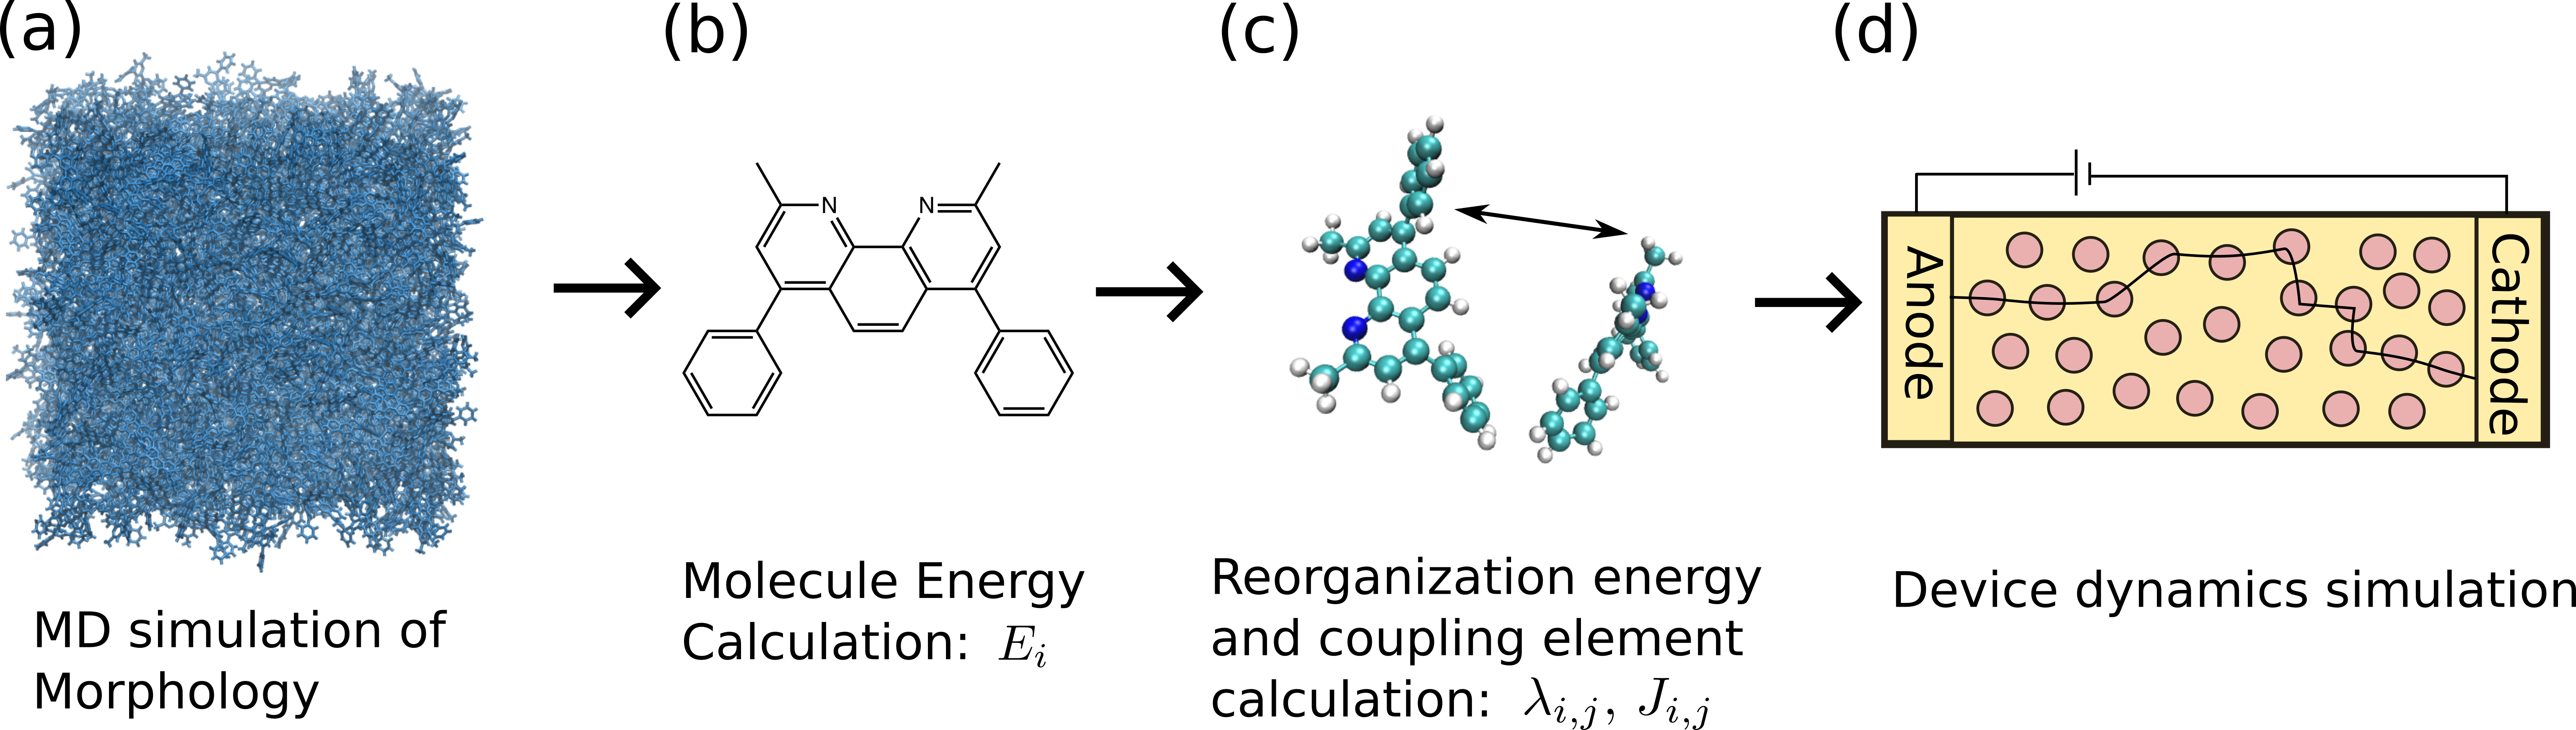
\includegraphics[width=0.95\textwidth]{figs/MSM.png}
    \caption{The multiscale model workflow for OSC. Step 1: MD simulation to generate atom coordinates. Step 2: Molecule energy $E_i$ calculation. Step 3: Calculation of Reorganization energy $\lambda_{i,j}$ and coupling element $J_{i,j}$ for pairs of molecule $i,j$ whose COM distance is less than $r_\text{cutoff}$. Step 4: Modelling dynamics on device level, such as ToF calculation.}
    \label{fig:MSM}
\end{figure}

Figure \ref{fig:scatterE} shows the workflow of the multiscale model for ToF calculation. In brief summary, the process includes: Firstly, classical Molecular Dynamics is used to generate the atomistic coordinates from which the vertex and edge sets are defined.
Specifically, using a cutoff distance $r_\text{cutoff}$, any two molecules whose center of mass (COM) within $r_\text{cutoff}=0.5$ [nm] form a pair of molecules where directed edge weight can be calculated.
Secondly, quantum electronic structure calculation is performed to obtain the electronic structure properties: The molecule energy $E_i$ of molecule $i$, the reorganization energy between $\left\{\lambda_{i,j}\right\}$ and coupling element $\left\{\Delta J_{i,j}\right\}$ between the pair of molecules $i$ and $j$. All in unit of eV. 

Then, those electronic structure properties are used to calculate the bi-molecular Marcus rate between the molecules:
%
\begin{equation}
    \omega_{ij} = \frac{2\pi}{\hbar} \frac{|J_{i,j}|^2}{\sqrt{4\pi \lambda_{i,j} k_\text{B}T}} \exp\left(-\frac{(\Delta E_{i,j} + q \vec{F} \cdot \vec{r}_{i,j} - \lambda_{i,j})^2}{4\lambda_{i,j} k_\text{B}T}\right) ,
    \label{equ:Marcus}
\end{equation}
%
where $\hbar$ is the reduced Planck constant, $k_\text{B}$ the Boltzmann constant. The temperature $T$ (in \unit[]{K}), external electric field $\vec{F}$ and the charge of the carrier $q$ (in \unit[]{e}) can be considered as parameters of the simulation. The vector $\vec{r}_{i,j} = (r^x_{ij},r^y_{ij},r^z_{ij})^\text{T}$ connects the center-of-masses of molecules $i$ and $j$, which is calculated using cyclic boundary conditions depending on system setting. And $\Delta E_{i,j} = E_i - E_j$ is the energy difference between a pair of molecules.
Finally, the quantity of interest, such as ToF $\tau$, can be calculated from the transition rates $\omega_{ij}$.

\subsection{Molecule Dynamics Simulation}
In a material system of $N_a$ atoms with mass and position denoted by $m_i$ and $\vec{r}_i$ respectively, molecular dynamics (MD) models the evolution of the atomic coordinate using Newton's second law, which is written in Hamilton equation: 
\begin{equation}
    \begin{cases}
        \frac{d \vec{r}_i}{dt} = \frac{\partial H }{\partial \vec{p}_i} \\
        \frac{d \vec{p}_i}{dt} = -\frac{\partial H }{\partial \vec{r}_i}
    \end{cases}
    \label{eq:Hamilton}
\end{equation}
for $i=1,\cdots,N_a$, where the Hamiltonian $H$ reads:
\begin{equation}
    H=\sum\limits_{i} \frac{|\vec{p}_i|^2}{2 m_i} + U(\vec{r}_1,\cdots,\vec{r}_{N_a})
    \label{eq:Hamilton2}
\end{equation} 

In principle the potential energy function $U(\vec{r}_1,\cdots,\vec{r}_{N_a})$ of the system can be obtained from electronic structure models. In practice, it is a very computationally expensive procedure, and without too much loss in precision, MD use empirical potentials that are designed for specific purposes.
In our work, constant the molecule number $N=1000$, a temperature $T=300$ K and a pressure at 1 atm is used to achieve an NPT ensemble. 
One of the final BCP morphology is chosen as OSC for charge transport study. 

\subsection{Electronic Structure Calculation} 
The molecule energy $E_i$ in the multiscale model is calculated as:
\begin{equation}
E_i = (U^\text{cC}_i - U^\text{nN}_i) + (E^\text{c}_i - E^\text{n}_i)
\label{eq:E_i}
\end{equation}
where $U^\text{cC}_i$ is the internal energy of charged molecule $i$ in the optimized charged geometry, and $U^\text{nN}_i$ is the internal energy of neutral molecule $i$ in the optimized neutral geometry. The calculation of $U$ and how to obtain optimized geometry will be introduced in the subsection DFT Calculation.
In the superscript the lowercase letter "c/n" represents the molecule state of being charged/neutral and uppercase letter "C/N" represents the geometry of the charged/neutral molecule. This notation also applies for $E^\text{c}_i$, $E^\text{n}_i$. 
And $E^\text{n}_i = E^\text{n,el}_i + E^\text{n,induce}_i$ is the energy due to the electrostatic and induced dipole moment effect. Compared with the electrostatic energy calculated using the dielectric constant, this energy in multiscale model is very sensitive to the molecule structure, making the uncertainty quantification of charge transport in multiscale model much more important. 
A precise method for calculating $E^\text{n}_i$ is to use the Thole Model as detailed in \cite{Baumeier2011}.

This method has the steps include: first, each atom $a_i$ is initialized with charges $q_{a_i}$ and dipole moment $D_{a_i}$. 
Then the induced dipoles of each atom are calculated using the electric field generated by other atoms $b_j$.
This calculation continuous iteratively to update the induced dipoles of every atom by considering the fields due to other dipoles.
Finally, it checks for convergence, if the induced dipoles have not changed significantly from one iteration to the next, the iterative process stops.
Finally, the electrostatic energy and polarization energy using the final set of induced dipoles and atomic charges. So in summary, $E^\text{n}_i$ is a function of all atoms' charges and induced dipoles: $E^\text{n}_i = \sum\limits_{a_i} f(q_{a_i}, D_{a_i})$. 

The reorganization energy $\lambda_{i,j}$ between molecule $i$ to molecule $j$ is given as:
\begin{equation}
    \lambda_{ij} = U_i^\text{nC} - U_i^\text{nN} + U_j^\text{cN} - U_j^\text{cC}
\end{equation}

%%%%%%%
The coupling element $J_{i,j}$ between molecule $i$ and $j$ is calculated \cite{baumeier_density_2010} using the electron wave function of the molecules obtained from the Kohn-Sham equation: 
\begin{equation}
    J_{i,j} = \frac{ J^0_{i,j}- \frac{1}{2}(e_i+e_j)S_{i,j} }{ 1- S_{i,j}^2 }
    \label{equ:JAB}
\end{equation}
where $J^0_{i,j} = \langle \psi^i | \hat{H} | \psi^j \rangle $, $e_i = \langle \psi^i | \hat{H} | \psi^i \rangle $, $e_j = \langle \psi^j | \hat{H} | \psi^j \rangle $, and $S_{i,j}=\langle \psi^i | \psi^j \rangle $ with bra-ket notation, $\hat{H}$ is the Hamiltonian of the electron wave function, and $\psi^{i,(j)}$ is the electron wave function of molecule $i(j)$. A single molecule is called a monomer, and a pair of two molecules is called a dimer.

Denote $\psi^\text{D}$ as the electron wave function of the two molecules,  $J^0_{i,j}$ can be calculated via:
$
    J^0_{i,j} = \mathbf{\gamma}^i \text{diag}(\mathcal{E}) \mathbf{\gamma}^j
$, 
where $\mathbf{\gamma}^i = \langle \psi^i | \psi^\text{D} \rangle$ and $\mathbf{\gamma}^j = \langle \psi^j | \psi^\text{D} \rangle$ are called the projections of the monomer orbitals $\psi^i, \psi^j$ on the dimer orbitals $\psi^\text{D}$. And $\text{diag}(\mathcal{E})$ is the diagonal matrix consisting of energy eigenvalues of the one-particle wave function of the dimer.

In conclusion, the calculation of electronic structure relies on the internal energy and electron wave function. As mentioned in the introduction, DFT is used to calculate these two quantities. The next subsection will introduce the details of DFT.

%%%%%%%%%%%%%%%%%%%%%%%%%%%%%%%%%%%%%%%%%%%%%%%%%
\subsection{DFT Calculation}
In multiscale model, each molecule is an $N_\text{el}$-electron system, and the probability of finding electrons in space is described by the wavefunction.
In DFT, the internal energy calculated from the Kohn–Sham equation \cite{kohn_self_1965} reads:

\begin{equation}
    U^\text{KS}[\rho] = T_s[\rho] + \int \hat{V}_\text{ext}(\vec{r}) \rho(\vec{r}) d \vec{r} + \hat{V}_\text{H}[\rho] + \hat{V}_\text{XC}[\rho]
    \label{eq:KS_model}
\end{equation}
where the electron density is $\rho=\sum\limits_{i=1}^{N_\text{el}} \phi_i^\star(\vec{r}) \phi_i(\vec{r})$, $T_s[\rho]$ is the kinetic energy depending on $\rho$,  $\hat{V}_\text{ext}$ is the external potential energy,  $\hat{V}_\text{H}[\rho]$ is the Hartree energy accounting for the Coulomb interaction, $\hat{V}_\text{XC}[\rho]$ is the exchange-correlation energy accounting for the difference between classical and quantum effect. The exact form of $\hat{V}_\text{XC}[\rho]$ is not known, in practice, this energy term is approximated by DFT functionals. In our work, ten DFT functionals are used to represent this energy term. 
The single-electron wave function $\phi_i$ satisfies: 
\begin{equation}
    (-\frac{1}{2}\nabla^2_{\vec{r}} + \hat{V}_\text{ext} + \frac{\delta \hat{V}_\text{H}[\rho]}{\delta \rho} + \frac{\hat{V}_\text{XC}[\rho]}{\delta \rho}) \phi_i^\text{KS}(\vec{r}) =  \epsilon^\text{KS}_i[\rho] \phi^\text{KS}_i (\vec{r}) 
    \label{eq:KS2}
\end{equation}
with $\epsilon^\text{KS}_i[\rho]$ being the energy eigenvalue of electron $i$. 
In practice, Equation \ref{eq:KS2} is solved iteratively, and the wave function is represented by a linear combination of basis functions call basic sets. 
In this work, the basic set def2-tzvp \cite{weigend_accurate_2006} is used. The DFT computation is performed by VOTCA \cite{Baumeier2011} which internally calls ORCA software.
The internal energy $U^\text{KS}$ depends on the atomic coordinates of the molecule. The optimized geometry of a molecule refers to the atomic coordinates that minimize $U^\text{KS}$.

\section{Time-of-flight Calculation}
The multiscale model defines a graph $\mathbf{G}$ with an adjacency matrix $\mathbf{W}$, where the edge weights $\omega_{i,j}$ represent the Marcus rate from molecule $i$ to molecule $j$. The charge dynamics are modeled as a continuous-time random walk on this graph. In the time-of-flight (ToF) model, some vertices serve as \textit{Source} nodes, representing the electrode where charge carriers are injected, and some as \textit{Sink} nodes, where charge carriers are detected and the ToF is recorded.

As mentioned in the introduction, a quantity of interest in modeling charge dynamics is the ToF, which is the time for charges carriers injected into the Source to be detected at the Sink.
A typical method to obtain the ToF is to use the kinetic Monte Carlo (KMC) method to simulate the CTRW for many times and record ToFs, which are random variables. 
To be detailed: 
But a challenge with this KMC is that one need to repeat a large number $N_\text{KMC}$ of KMC simulation to guarantee an converged ToF. Furthermore, $N_\text{KMC}$ is not known before running KMC, posing a great challenge to quantify the uncertainty of ToF from the multiscale model. 
An alternative method to overcome the convergence challenge is to obtain ToF as the hitting time a continuous time Markov chain.

Due to Pauli repulsion, each node can be occupied by at most one charge carrier. For a system with $N$ molecules and $N_c$ charge carriers, there are ${N \choose N_c}$ possible occupation states. Each occupation state is denoted as $\mathbf{s}$. A state is called the Source state if all carriers occupy the Source nodes, and a Sink state if at least one of the Sink nodes is occupied.

The transition rates between the states can be obtained from the adjacency matrix $\mathbf{W}:\omega_{i,j}$, since the connectivity of states is encoded in the connectivity of the nodes, as detailed in ~\cite{chen_graph_2024}. 
According to such connectivity, 
the transition rates $\Omega_{\mathbf{s} \mathbf{s}' }$ from state $\mathbf{s}$ to $\mathbf{s}'$ is:
\begin{equation}\label{eq:transition_rates}
	\Omega_{\mathbf{s} \mathbf{s}^\prime} =
	\begin{cases}
	     0			&  \mathbf{s} \text{ is not connected to } \mathbf{s}^\prime,\\
	    \omega_{ij}	&  \mathbf{s} \text{ is connected to } \mathbf{s}^\prime \text{ due to } (i,j)
	\end{cases}
\end{equation}

Then the transition probability from state $\mathbf{s}$ to $\mathbf{s}'$ is $p_{\mathbf{s} \mathbf{s}^\prime} = \Omega_{\mathbf{s} \mathbf{s}^\prime}/D_\mathbf{s}$ where $D_\mathbf{s} := \sum_{\mathbf{s}^\prime \ne \mathbf{s}} \Omega_{\mathbf{s} \mathbf{s}^\prime}$.
And the expected time from state $\mathbf{s}$ to reach the Sink state $\tau_\mathbf{s}$ is calculated via: 
\begin{equation}\label{eq:hitting_time}
	\tau_\mathbf{s} = \begin{cases}
		\frac{1}{D_\mathbf{s}} + \sum_{\mathbf{s}^\prime \ne \mathbf{s}} p_{\mathbf{s} \mathbf{s}^\prime} \tau_{\mathbf{s}^\prime} &\text{if $\mathbf{s}$ is not a sink state},\\
		0 &\text{else.} 
	\end{cases}
\end{equation} 

To account for all possible starting nodes of the carriers, all Source states must be considered. The random walk process can be modeled as a parallel electric network of capacitors \cite{doyle_random_2000}. Accordingly, the ToF is evaluated using the harmonic mean:
\begin{equation} 
\tau = N_\text{source} \left[\sum_{\mathbf{s} \in \text{Source}} (\tau_\mathbf{s}^\ast)^{-1}\right]^{-1},
\label{eq:ToF}
\end{equation}
where $N_\text{source}$ is the number of Source states.

%%%%%%%%%%%%%%%%%%%%%%%%%%%%%%%%%%%%%%%
\section{Results on BCP}
\label{sec:result}

A OSC device consisting of 1000 BCP molecules arranged in $8 \times 8 \times 8$ cubic box is simulated using MD, as shown in Fig. \ref{fig:MSM}(a).
The \textit{Source} contains molecules whose COM have X-coordinates $0 < r^x_i < 0.5$ nm, and \textit{Sink} molecules $7.5 < r^x_i < 8$. 
This section presents the molecule energy distribution, coupling element distribution, reorganization energies and ToFs calculated using the 12 DFT functionals. 
Using the PBE0 functional as a reference, the difference in electronic structure distributions due to DFT functionals is measured by the Wasserstein distance. In contrast to the small Wasserstein distance between the electronic structure distributions, the difference in ToF $\Delta \tau$ is relatively large. 
Next, the change of the graph connectivity due to different DFT functionals is used to explain the $\Delta \tau$.
Following this, a normal distribution estimated from maximum likelihood is used to represent the uncertainty in each electronic structure parameters. Then distributions of ToF are obtained using the electronic structure parameters generated by Monte Carlo sampling from the estimated distributions. Finally, the sensitivities of $E_i,J_{i,j},\lambda_{i,j}$ to ToF are compared, confidence level of ToFs are estimated. 

\subsection{Electronic Structure Parameters and ToFs}
Using ten different functionals, the molecule energies, coupling elements and reorganization energies are calculated from the multiscale model with ten different DFT functional.

Table \ref{tab:para} summarizes the names of the DFT functionals, the amount of Hartree-Fock exchange (HFX), the reorganization energies, ToFs, the standard deviation of the molecule energy distributions, the drift ToFs under an electric field $6 \times 10^7$ V/m and mobility.
The table indicates that while the energy standard deviations $\sigma(E)$ are similar across different functionals, the ToF vary significantly, notably for functionals like BHANDHLYP, M06L, and BHLYP.

\begin{table}[h]
    \centering
    \begin{tabular}{c c c c c c c}
    \hline
        Functional & HFX & $\lambda_{i,j}$ [eV] & ToF [s] & $\sigma(E)$ & drift ToF [s] & $\mu$ [m/s] \\ 
        \hline
        PBE0 & 0.25 & 0.388 & $1.23\times 10^{-3}$ & 0.175 & $1.44 \times 10^{-6}$ & $9.40\times 10^{-7}$ \\
        PBE & 0 & 0.303 & $1.04\times 10^{-3}$ & 0.172 & $2.27 \times 10^{-7}$ & $5.95 \times 10^{-6}$ \\ 
        B3LYP & 0.20 & 0.375 & $4.28\times 10^{-3}$ & 0.175  & $3.22\times 10^{-7}$ & $4.08 \times 10^{-6}$ \\
        BHANDHLYP & 0.5 & 0.494 & \textbf{737.94} & 0.192  & $4.75\times 10^{-2}$ & $2.86\times 10^{-11}$ \\
        TPSS & 0 & 0.310 & $1.37\times 10^{-2}$ & 0.168  & $1.03 \times 10^{-6}$ & $1.30\times 10^{-7}$ \\
        BP86 & 0 & 0.304 & $7.46\times 10^{-3}$ & 0.175  & $5.81 \times 10^{-7}$ & $2.33\times 10^{-6}$ \\
        wB97X & 0.157 & 0.505 & $2.92\times 10^{-2}$ & 0.191  & $2.01\times 10^{-6}$  & $6.74\times 10^{-7}$ \\
        wB97X-D3 & 0.195 & 0.496 & $4.89\times 10^{-2}$ & 0.180  & $2.50 \times 10^{-6}$ & $5.42 \times 10^{-7}$ \\
        M06L & 0 & 0.312 & 0.319 & 0.165 & $2.11 \times 10^{-5}$ & $6.42 \times 10^{-8}$ \\
        BHLYP & 0.5 & 0.493 & 2.47 & 0.192  & $5.96 \times 10^{-5}$ & $ 2.28\times 10^{-8}$  \\
    \hline
    \end{tabular}
    \caption{DFT functional HF exchange scaling (HFX), calculated values of reorganization energy ($\lambda_{i,j}$), diffusive ToF, energy disorder ($\sigma(E)$), drift ToF, and mobility ($\mu$) for BCP molecules for different DFT functionals.}
    \label{tab:para}
\end{table}

The functional BHANDHLYP gives a ToF much larger than the rest of the 9 functionals. 
The reason for this large ToF in BHANDHLYP is that one molecule has relatively low energy, and the out-going rate for this molecule is very small, eventually leading to large ToF. 
However, such large difference in a material system is non-physical, and studying the uncertain quantification based on those ToF data can not indicate anything on the robustness of the multiscale model. 

A noticeable difference in all the different functional is the amount of HF for approximating the exchange-correlations. 

So by fixing the functional to be the commonly used PBE0 functional, the HFX is varied to investigate the effect of HFX to the molecular properties and ToF. 
Hybrid functionals like PBE0 or B3LYP use a specific, empirically determined fraction of HF exchange that generally works well for a broad range of applications.
PBE0 is constructed by combining 25\% of the exact exchange from HF theory with 75\% of the exchange from the Perdew-Burke-Ernzerhof (PBE) GGA exchange functional, along with the full PBE correlation functional.

When correlation effects are strong and electron-electron interactions play a significant role in determining their physical properties, the exact exchange overly localize electrons, and a lower HFX percentage or even pure DFT might perform better.
The $\pi$-electron conjugation and interactions in OSC such as BCP and MADN leads to significant electronic correlation effects within those materials. 

\subsection{BCP molecule with different HFX}
So our first investigation use the range of HFX=$0.05,0.15,0.23,0.24,0.25,0.26,0.27,0.35,0.45,0.55$. The values of HFX=$0.23,0.24,0.26,0.27$ are used because we want to see if a small perturbation in HFX would affect ToF significantly. 

Since ToF is sensitively affected by site energy, which is affected by the isotropic polarizability $P_\text{iso}$ and dipole moment $\mu$ of the molecules, we plot the those molecular properties as a function of HFX. 
\begin{figure}[h]
    \centering
    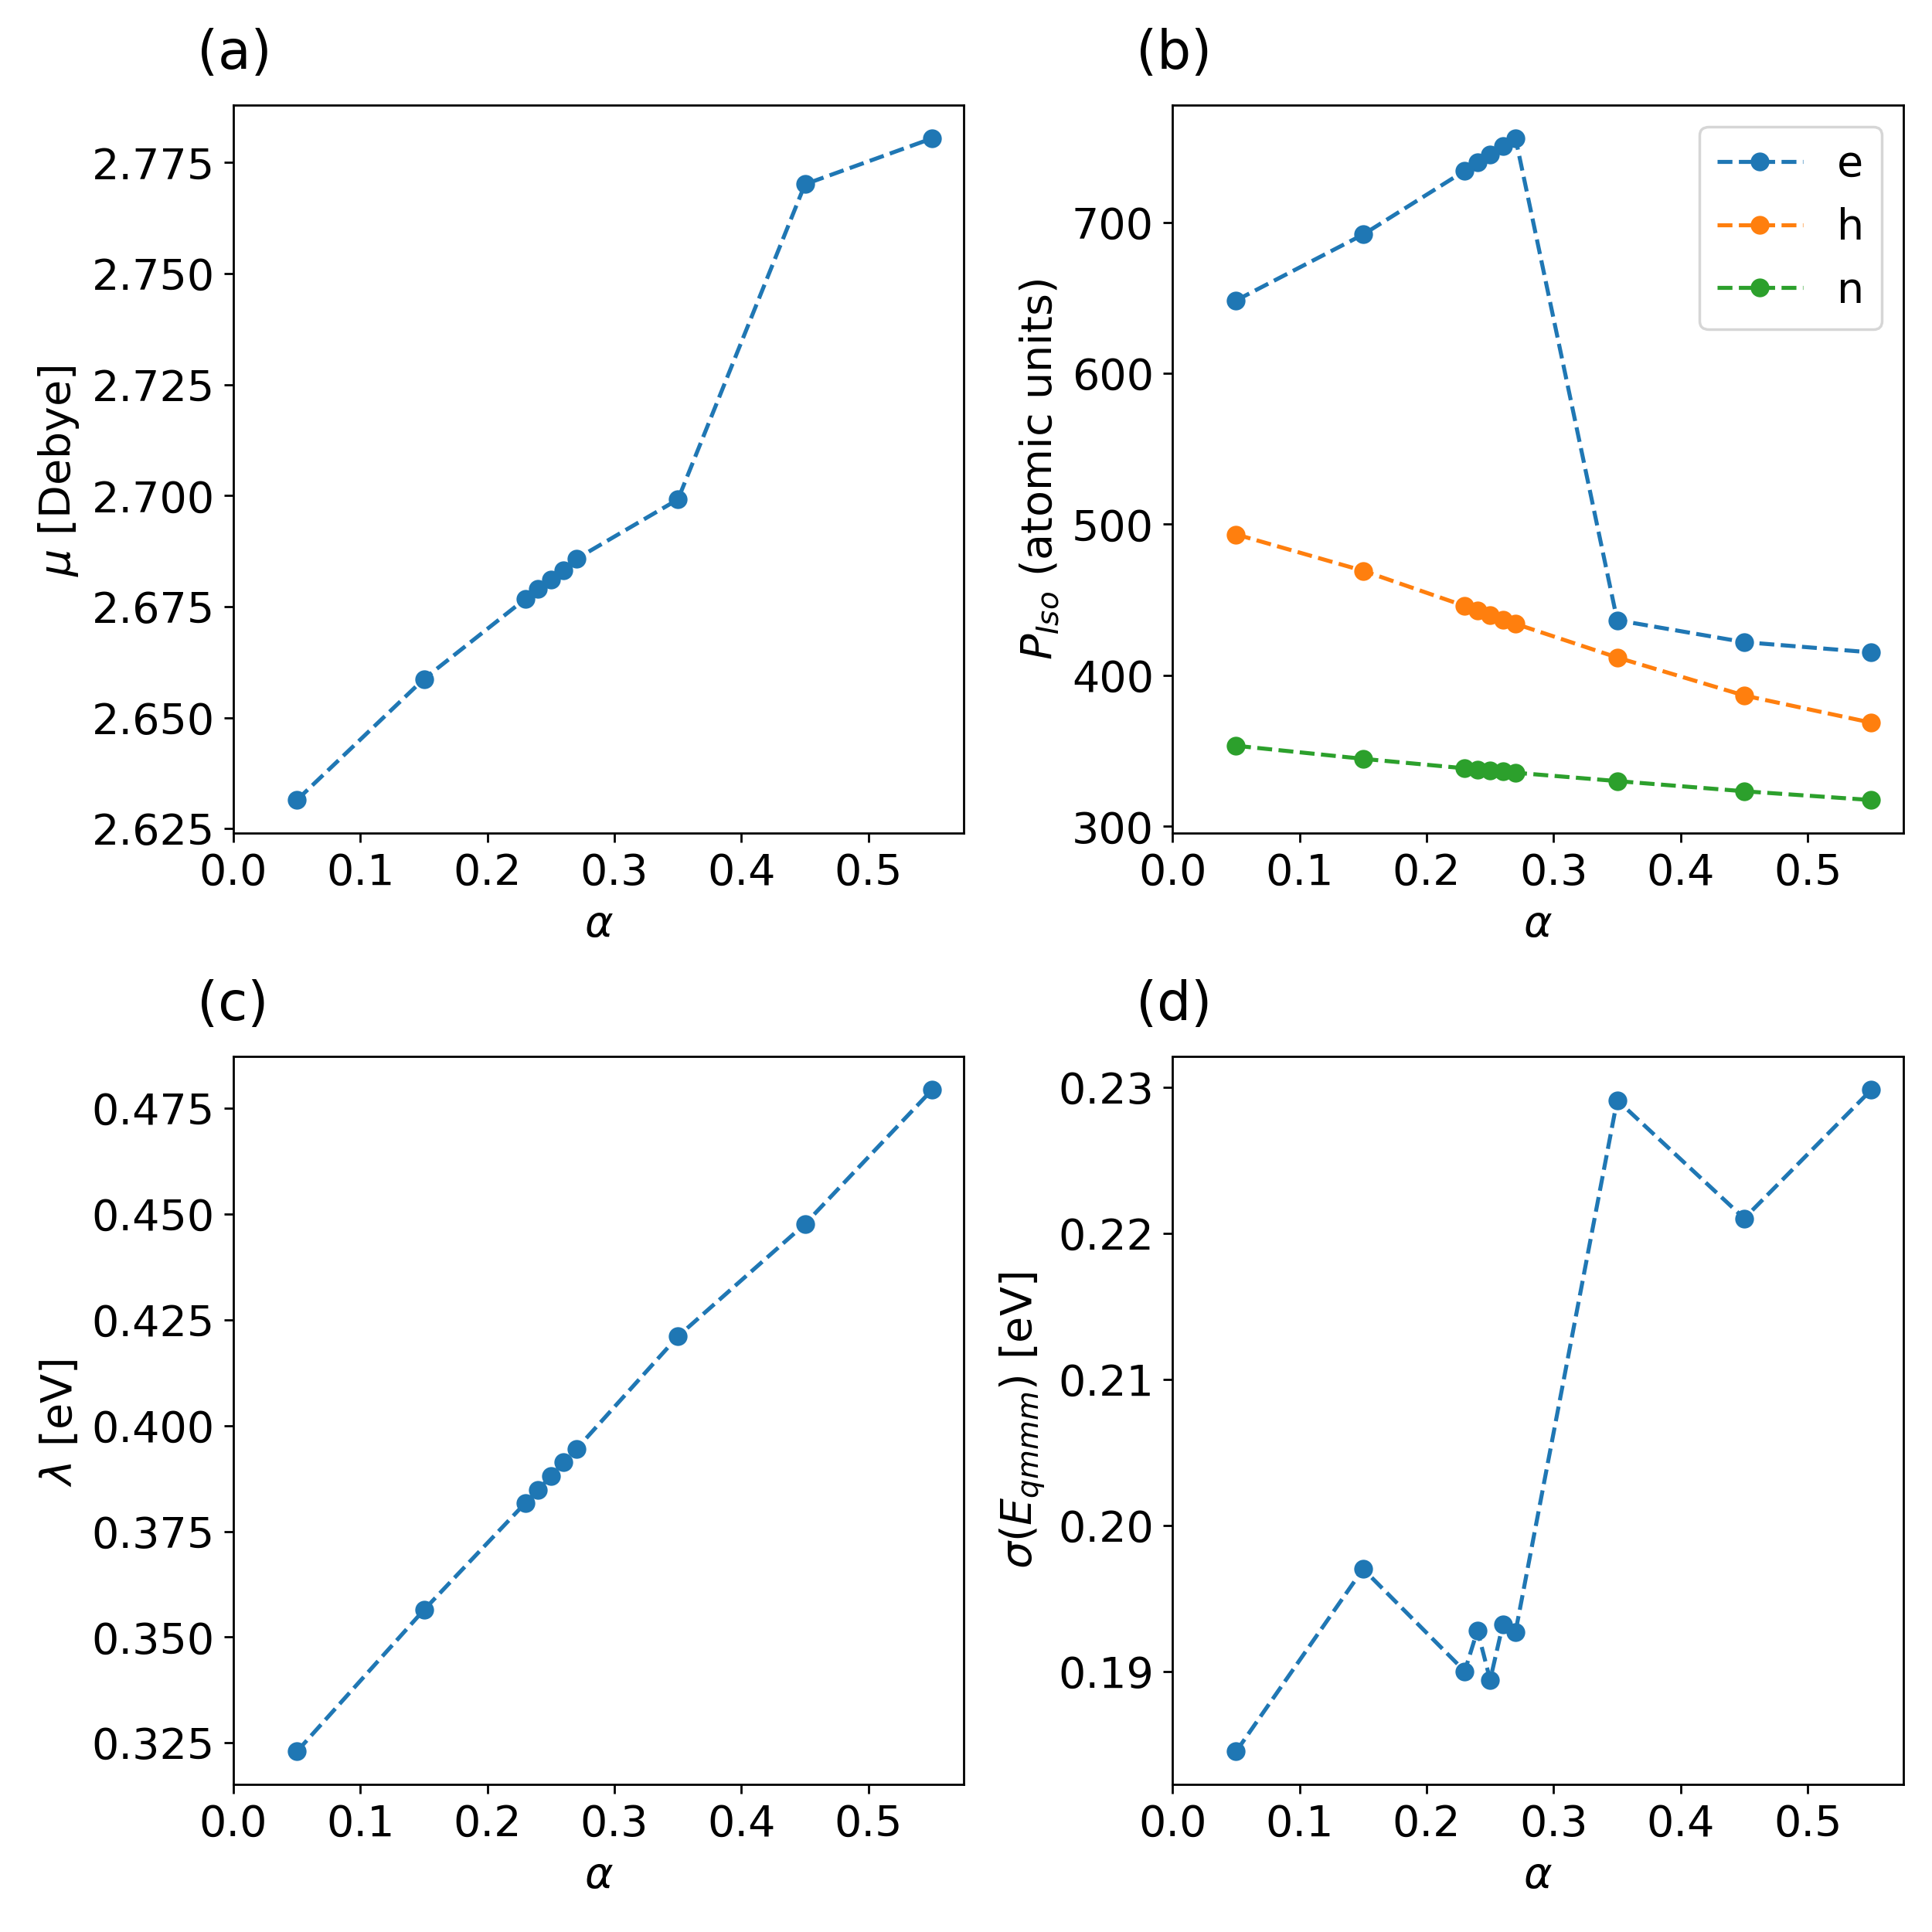
\includegraphics[width=0.9\textwidth]{figs/BCP_HFX/fig_autogen_BCP.png}
    \caption{(a) The neutral state BCP molecule dipole moment $\mu$, (b) isotropic polarizability $P_\text{iso}$, (c) reorganization energies $\lambda$ and (d) energy disorder $\sigma(E)$ as a function of the HFX parameters. }
    \label{fig:autogen}
\end{figure}
The Fig.\ref{fig:autogen}(a) shows that as HFX increase, the dipole moment increases first linear in the range of HFX=0.05 to 0.35, then a relatively large increase at HFX=0.35 to 0.55.
 
Figure \ref{fig:autogen}(b) shows that as HFX increase, the n state and h state BCP molecule has decreasing isotropic polarizability, showing that the molecule is getting more difficult to be polarized. 
Since the isotropic polarizability is decreasing as HFX increases, the screening effects are weaker for large HFX. 

Fig.\ref{fig:autogen}(c) shows that as HFX increase, reorganization energies are higher. Since the molecule requires more energy to reorient itself during the charge transfer process, the higher reorganization energy can slow down charge transport by making it energetically more costly for charges to move between molecules.

Fig.\ref{fig:autogen}(d) shows that when HFX=0.05-0.3 the energy disorder is relatively small (less than 0.2 eV). When HFX=0.35-0.55, the energy disorder $\sigma(E)>0.22$. 

The ToF of the BCP molecular system calculated using different HFX is shown in table \ref{tab:ToF_BCP_HFX}. This table shows that for HFX=0.35,0.45,0.55, the ToFs are extremely large compared to the ToFs for HFX<0.3. 
In contrast to the almost linear HFX-$\lambda$ relationship, those large ToFs are not physical. 


\begin{table}[h]
    \centering
    \begin{tabular}{c c c }
    \hline
        HFX & ToF [s] & ToF(no $E$) [s] \\
    \hline
        0.05 &  0.32010 & $3.004 \times 10^{-10}$ \\
        0.15 & 0.3879 & $4.668 \times 10^{-10}$ \\
        0.23 & 0.0200 & $6.787 \times 10^{-10} $ \\
        0.24 & 0.02977 & $7.0290 \times 10^{-10} $ \\
        0.25 & 0.02648 & $7.633 \times 10^{-10}$ \\
        0.26 & 3.259 & $7.824 \times 10^{-10}$ \\
        0.27 & 0.0359 &  $9.162 \times 10^{-10}$ \\
        0.35 & $1.72 \times 10^7 $ & $1.00 \times 10^{-9}$ \\
        0.45 & $1.8 \times 10^4$ & $1.32\times 10^{-9}$ \\
        0.55 & $1.23 \times 10^9 $ & $1.880 \times 10^{-9} $ \\
    \hline
    \end{tabular}
    \caption{The ToF with and without energy disorder of the BCP system as a function of the HFX. }
    \label{tab:ToF_BCP_HFX}
\end{table}


The reason for this non-physical ToF is that the site energy calculation use the atomic charges and molecular polarizability from the optimized BCP structure. However, each molecule in the BCP system has its own topology with different atomic charges and polarizability compared to the optimized BCP structure.  
Those difference in atomic charges and polarizability affect the site energy calculations. 

So the atomic charges and polarizability in the optimized structure can not be transferred to the BCP molecules generated from the MD simulation. 
For very disorder material system such as BCP, using the atomic charges and polarizability in the optimized structure can result in site energies that are deviated from the majority of the molecules. 

\begin{figure}[h]
    \centering
    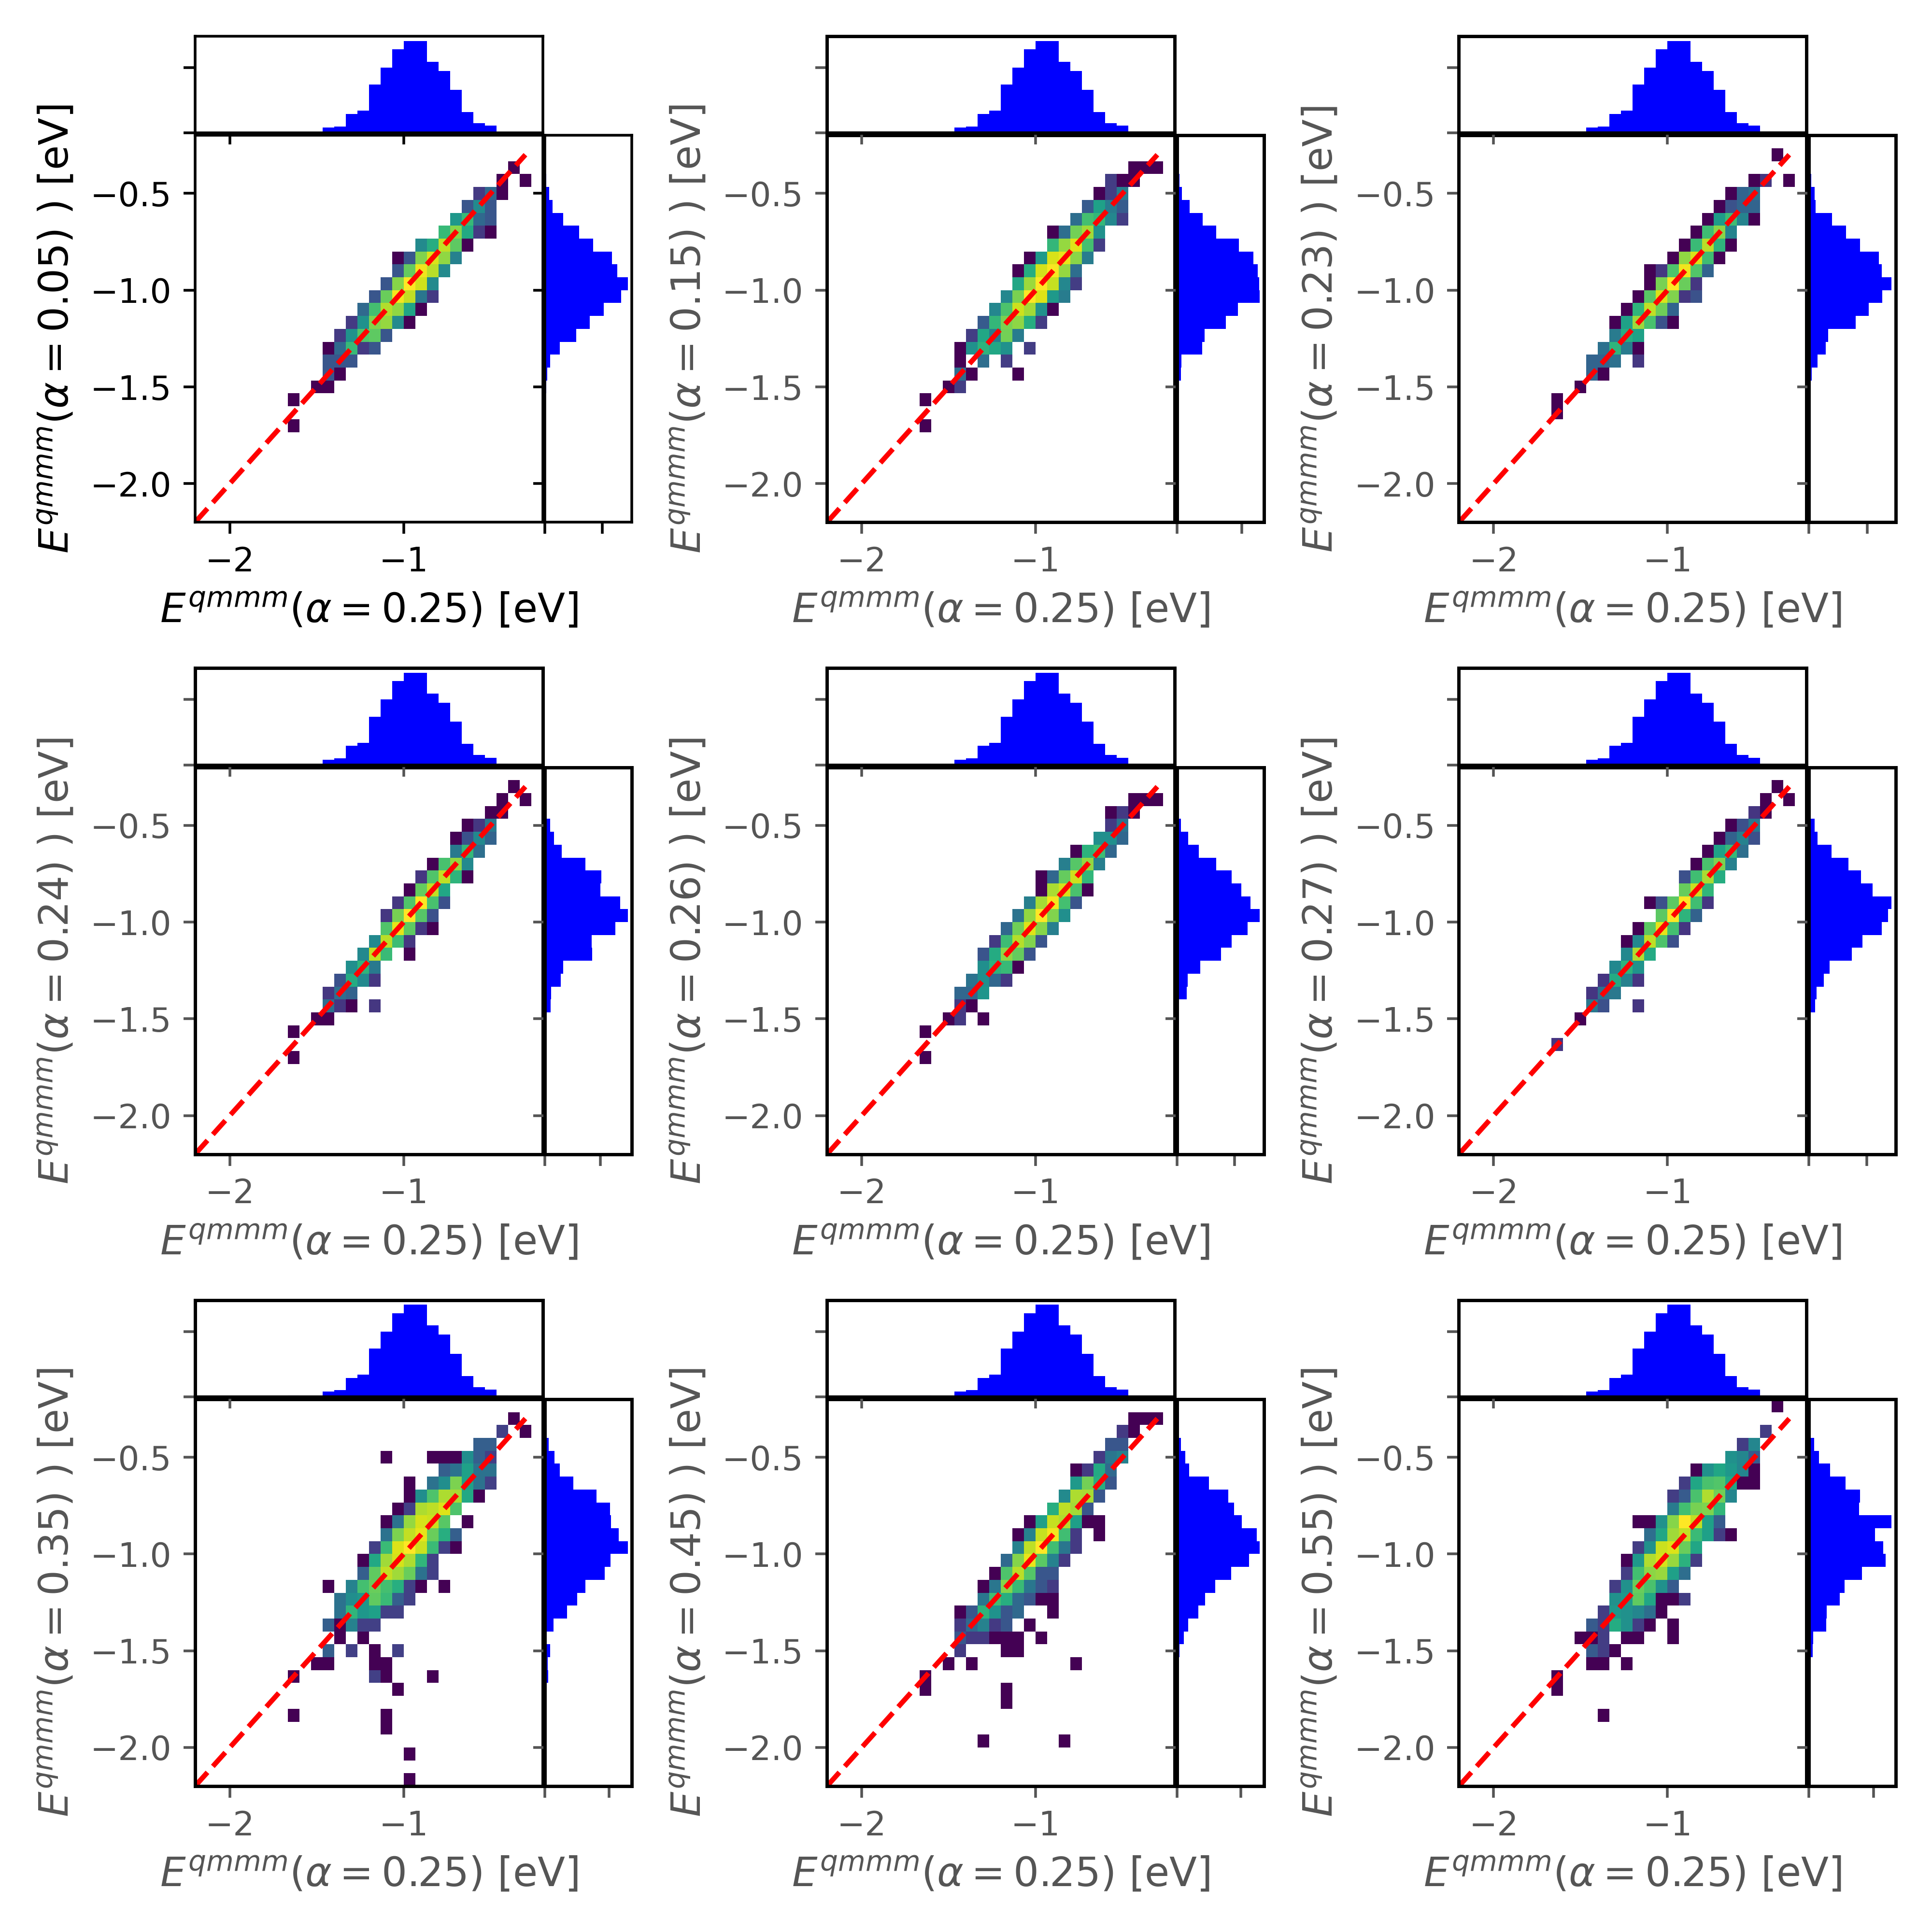
\includegraphics[width=0.95\textwidth]{figs/BCP_HFX/scatterE_qmmm.png}
    \caption{Scatter plot of site energy calculated from different HFX, compared to the site energy calculated from HFX=0.25 (The PBE0 functional). The brighter color near the diagonal lines indicates denser population of the molecules.  The top and right histogram show the energy distributions.}
    \label{fig:E_qmmm_BCP}
\end{figure}

Figure \ref{fig:E_qmmm_BCP} shows that for HFX<0.3, the site energies of all molecules are relatively close to the site energy obtained from PBE0 functional. When HFX=0.35, 0.45, 0.55, there are obvious low-energy molecules. 
Those low molecules results in the large energy disorder $\sigma(E)$ as shown in table \ref{tab:para}. 
For those three systems the ToFs are extremely large. 

The site energy has the contribution from the electrostatic effect and polarization effect due to the dipole moment of the molecules. 
The Heat map of the electrostatic energy and polarization energy are shown in Fig.\ref{fig:Estat_qmmm_BCP} and Fig.\ref{fig:Edip_qmmm_BCP}. 

Figure \ref{fig:Estat_qmmm_BCP} shows that for all HFX parameters, the electrostatic energy are relatively close, while Fig.\ref{fig:Edip_qmmm_BCP} shows that for HFX=0.35,0.45,0.55, there are molecules that have small polarization energy, contributing to the small site energies, and the extremely large ToF. 
Those small polarization energies and site energies are not physical. 
When HFX is varied, the change of the polarizability and reorganization energy are almost linear, while there is huge jumps in those site energies due to the huge jumps in the polarization energy. 

So for correlated system such as OSCs, large range of HFX leads to non-physical results. 
In the next section, we will use the range with small HFX values for the investigation of a less disorder molecular system, MADN. 

\begin{figure}[h]
    \centering
    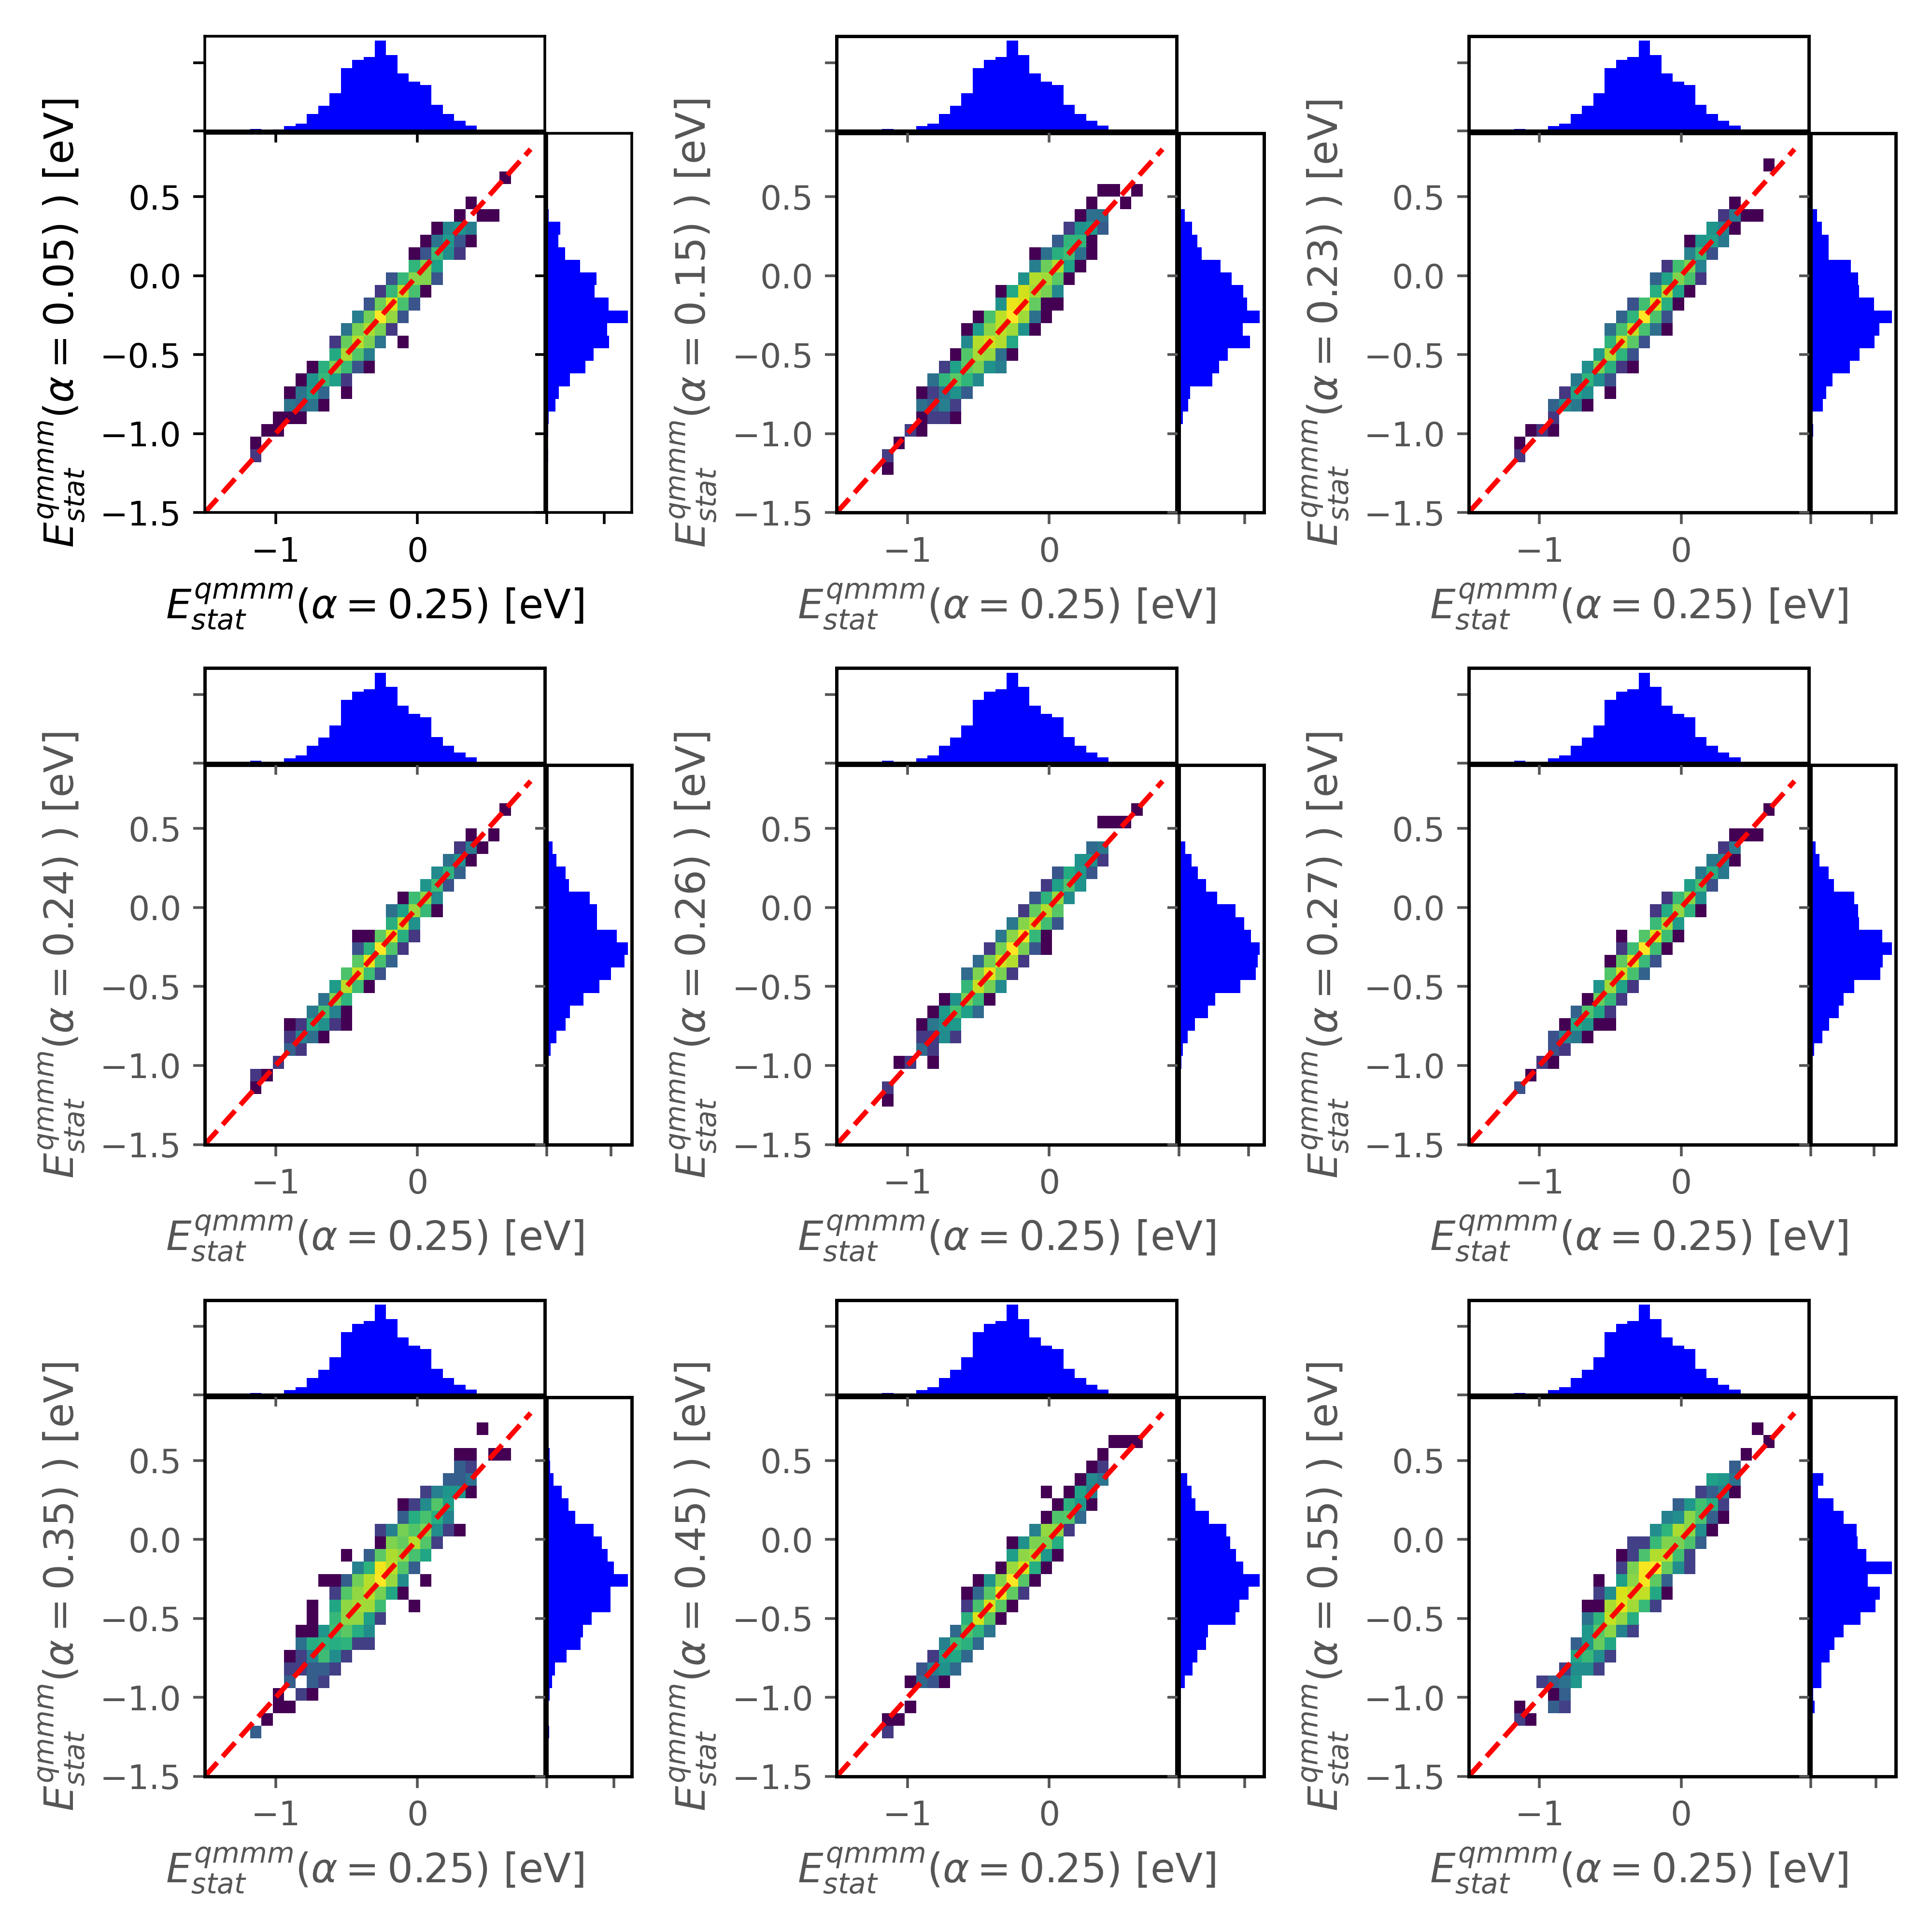
\includegraphics[width=0.95\textwidth]{figs/BCP_HFX/scatterEstat_qmmm.png}
    \caption{Scatter plot of electrostatic energy calculated from different HFX, compared to the electrostatic energy calculated from HFX=0.25 (The PBE0 functional). The brighter color near the diagonal lines indicates denser population of the molecules.  The top and right histogram show the energy distributions.}
    \label{fig:Estat_qmmm_BCP}
\end{figure}

\begin{figure}[h]
    \centering
    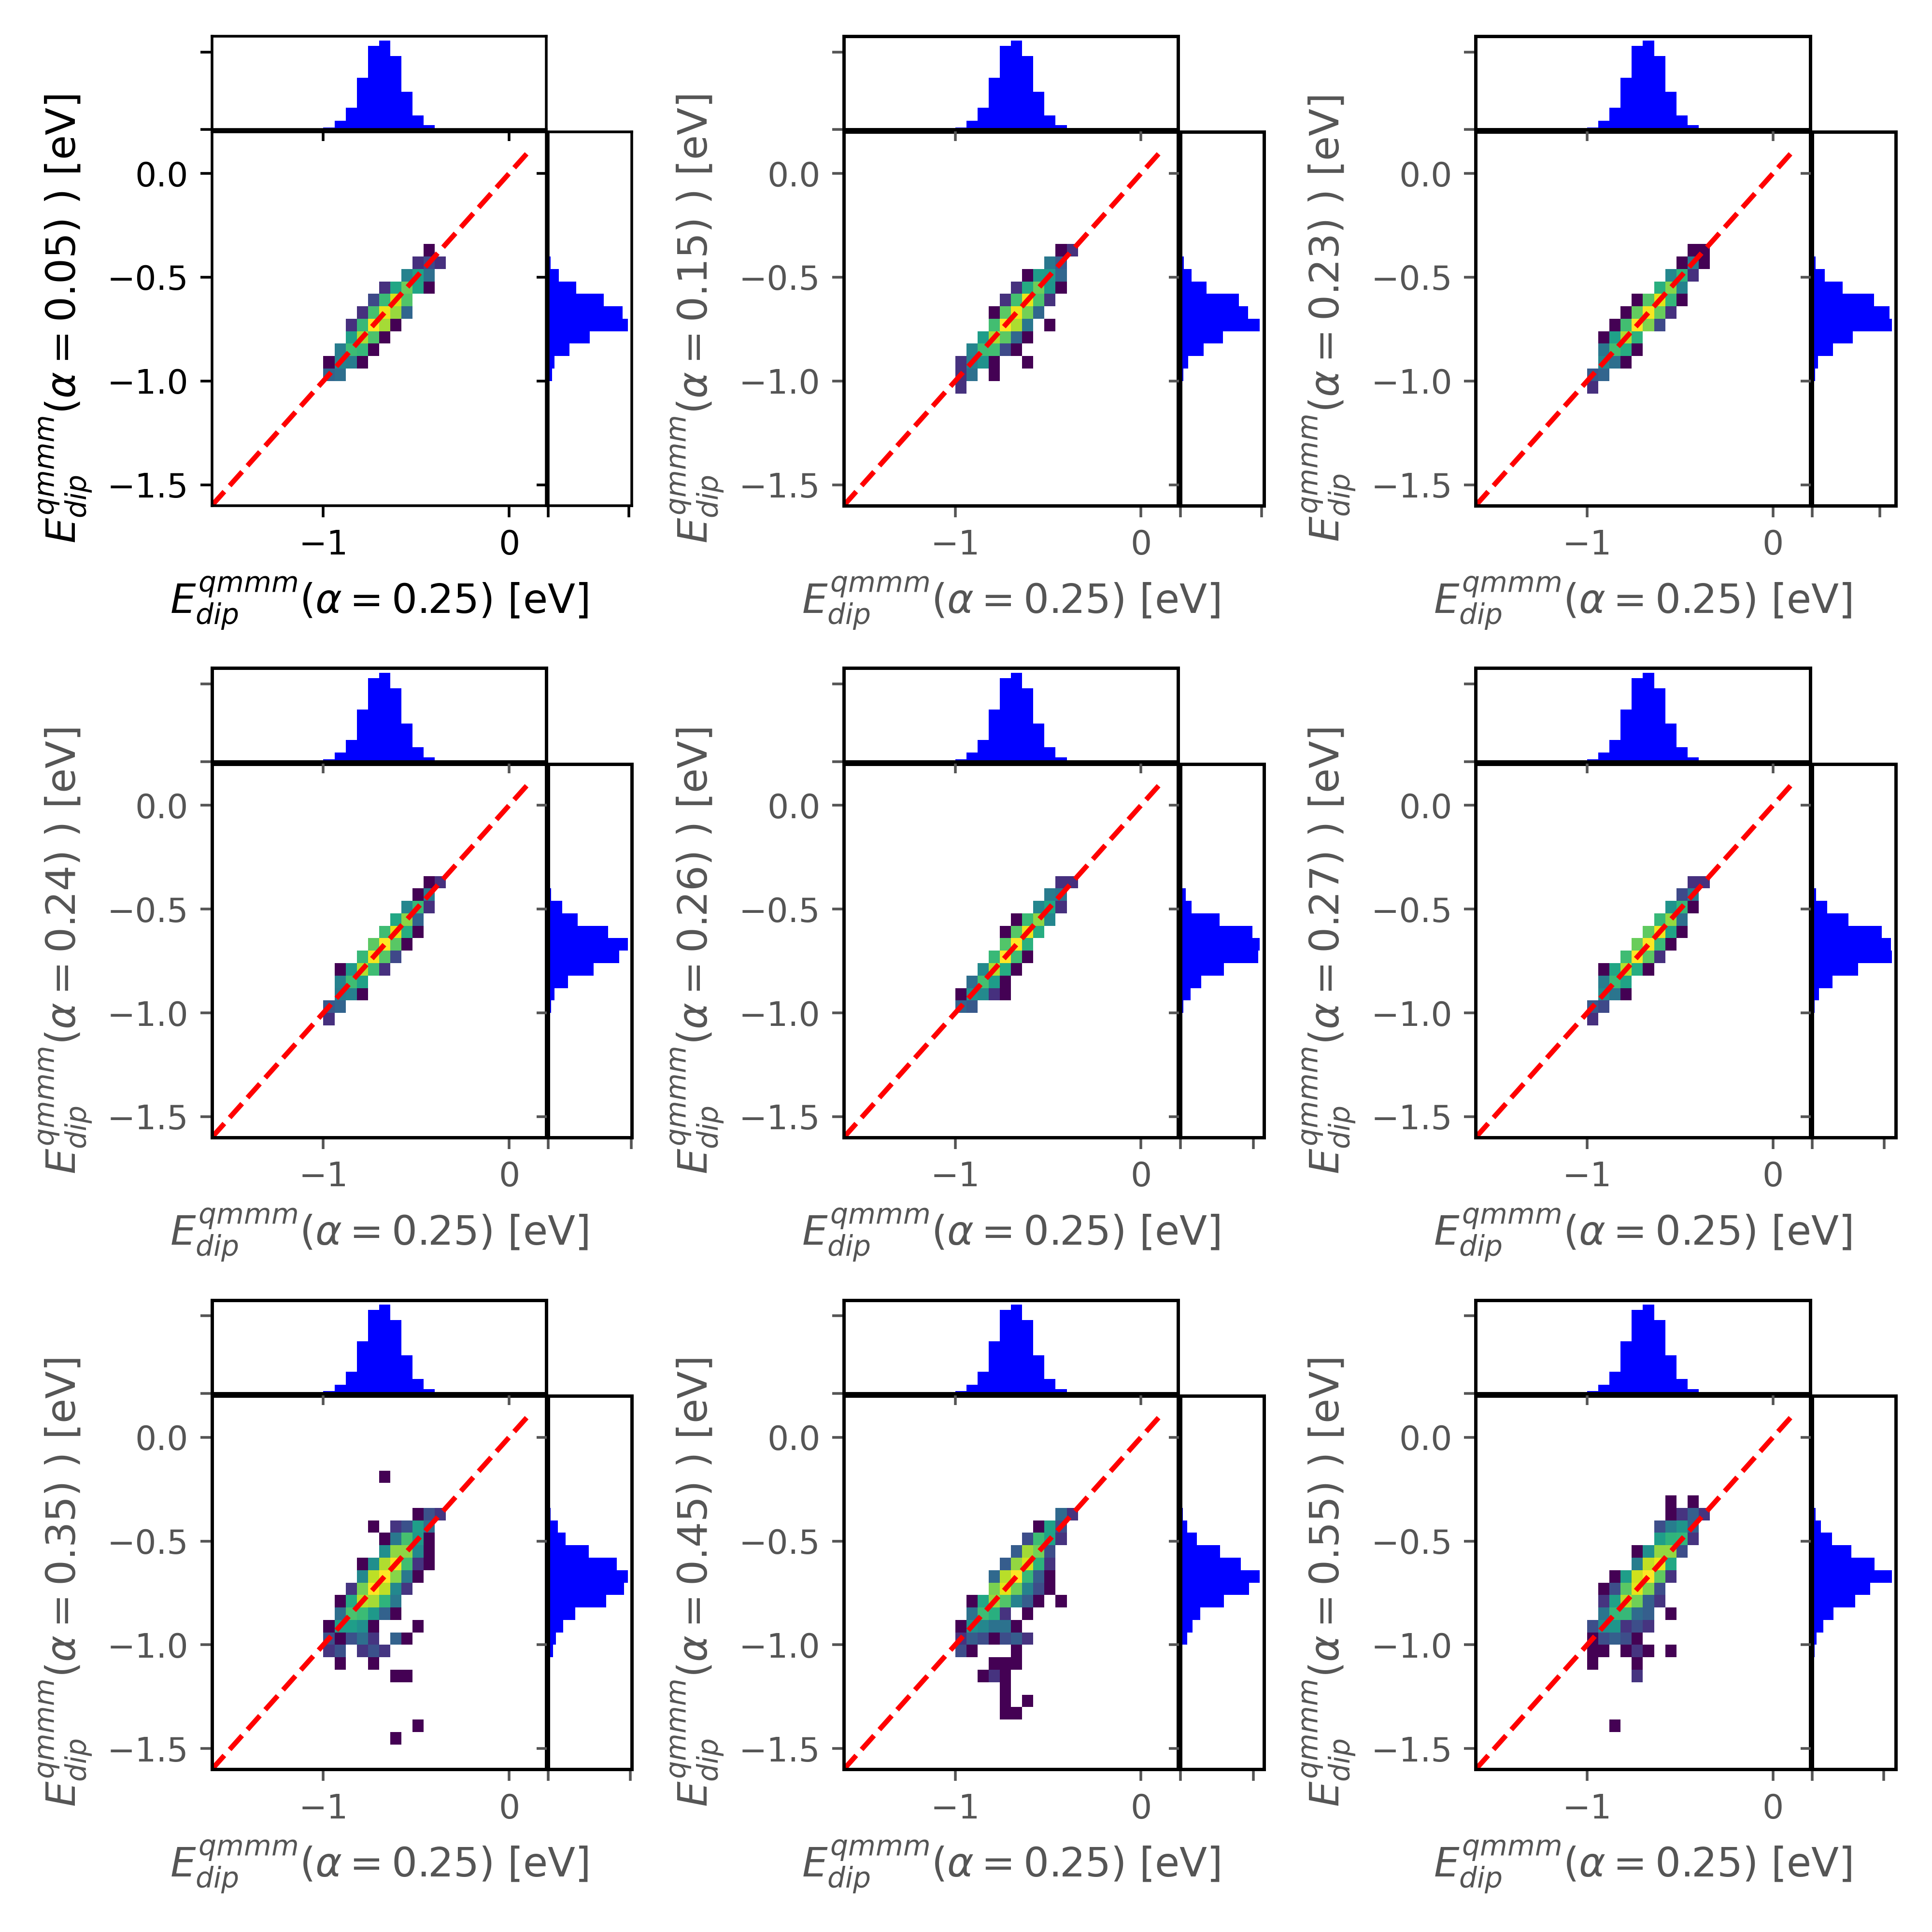
\includegraphics[width=0.95\textwidth]{figs/BCP_HFX/scatterEdip_qmmm.png}
    \caption{Scatter plot of polarization energy calculated from different HFX, compared to the polarization energy calculated from HFX=0.25 (The PBE0 functional). The brighter color near the diagonal lines indicates denser population of the molecules.  The top and right histogram show the energy distributions.}
    \label{fig:Edip_qmmm_BCP}
\end{figure}

\section{Results on MADN}
MADN (2-Methyl-9,10-di(naphth-2-yl)anthracene) is another type of OSC. 
The ToFs with and without energy disorder for HFX = 0.0, 0.05, 0.10, 0.15, 0.20, 0.25 are shown in 
\begin{table}[h]
    \centering
    \begin{tabular}{c c c }
    \hline
        HFX & ToF [s] & ToF(no $E$) [s] \\
    \hline
        0.00 &  $6.41 \times 10^{-9}$ & $1.88 \times 10^{-10}$ \\
        0.05 & $ 6.37 \times 10^{-9}$ (estimate) & $2.63 \times 10^{-10}$ \\
        0.10 & $ 1.74 \times 10^{-8}$ (estimate) & $3.31 \times 10^{-10} $ \\
        0.15 & $ 3.03 \times 10^{-8}$ & $3.96 \times 10^{-10} $ \\
        0.20 & $ 2.61 \times 10^{-8}$ (estimate) & $7.06 \times 10^{-10}$ \\
        0.25 & $ 9.54 \times 10^{-8}$ & $7.24 \times 10^{-10}$ \\
    \hline
    \end{tabular}
    \caption{The ToF with and without energy disorder of the MADN system as a function of the HFX. }
    \label{tab:ToF_MADN_HFX}
\end{table}



\bibliographystyle{unsrt}
\bibliography{references}





\begin{comment}
\textbf{Point 1:} To investigate the effect of different functionals $f^\text{DFT}$ on electronic structures, we compare the energies $E_i$ and couplings $J_{i,j}$ for all molecule indices $i,j$. Scatter plots in Figures \ref{fig:scatterE} and \ref{fig:scatterJ} illustrate these comparisons.

\begin{figure}[h]
    \centering
    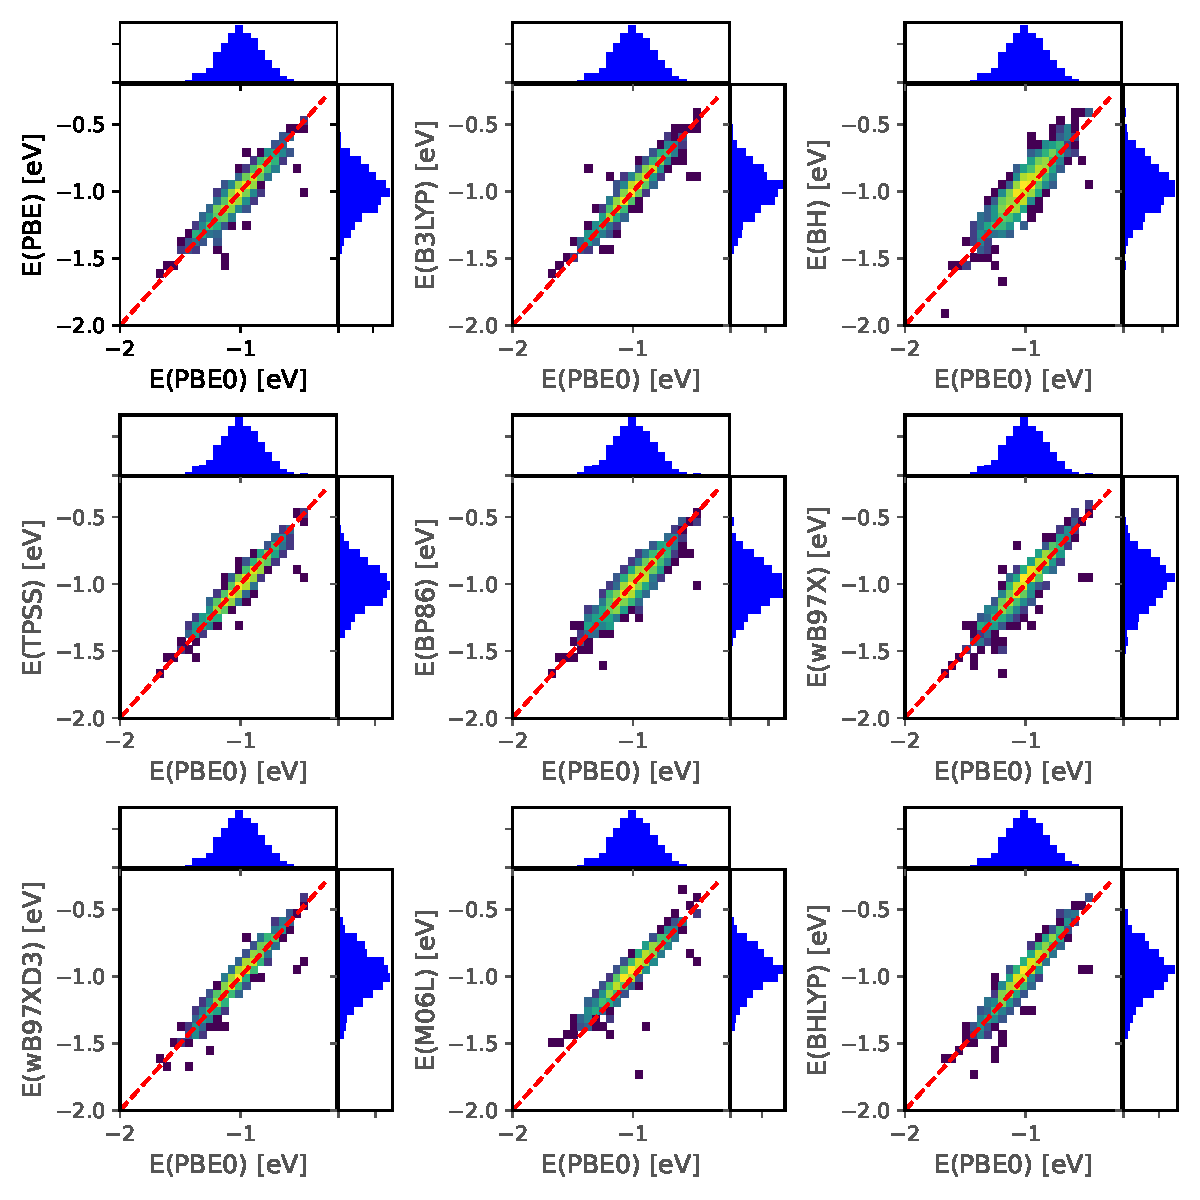
\includegraphics[width=0.95\textwidth]{figs/scatterE_all.pdf}
    \caption{Energy heat maps: $X$-axis shows energies of BCP molecules obtained using PBE0, while the $Y$-axis shows energies from a different functional $f'$.}
    \label{fig:scatterE}
\end{figure}

\begin{figure}[h]
    \centering
    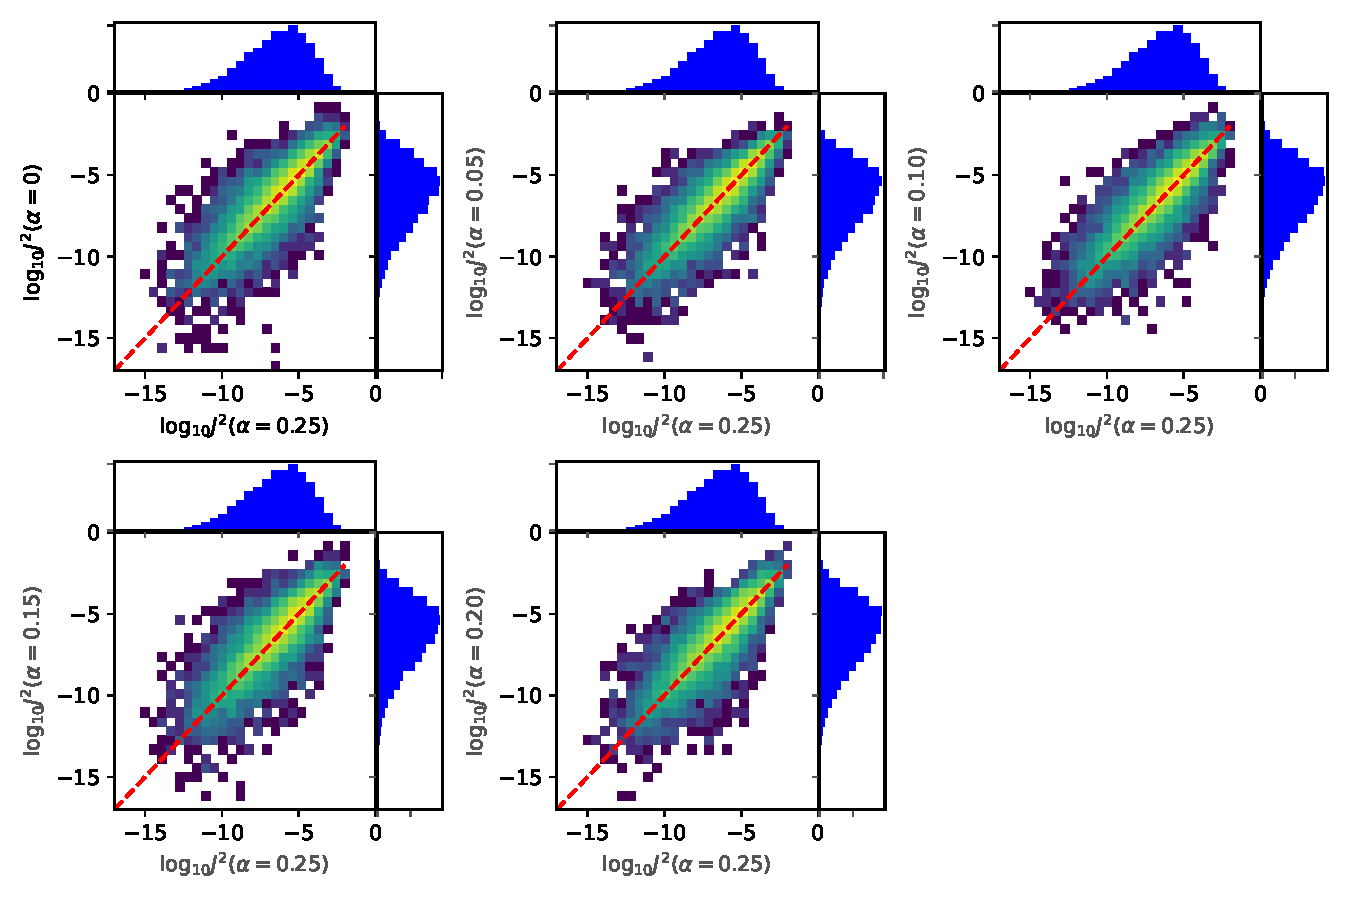
\includegraphics[width=0.95\textwidth]{figs/scatterJ_all.pdf}
    \caption{Scatter heat maps of $\log_{10}(J^2)$: $X$-axis shows $\log_{10}(J^2)$ of BCP molecules obtained using PBE0, while the $Y$-axis shows $\log_{10}(J^2)$ from a different functional $f'$.}
    \label{fig:scatterJ}
\end{figure}

\textbf{Point 2:} Both $E_i$ and $J_{i,j}$ are distributions. To quantify the impact of these distributions on $\Delta$ToF, we plot the Wasserstein distance versus $\Delta$ToF. Figure \ref{fig:distance_ToF} shows that different functionals generate similar energy sets, but $\Delta$ToF is not correlated with energy distribution distance.

\begin{figure}[h]
    \centering
    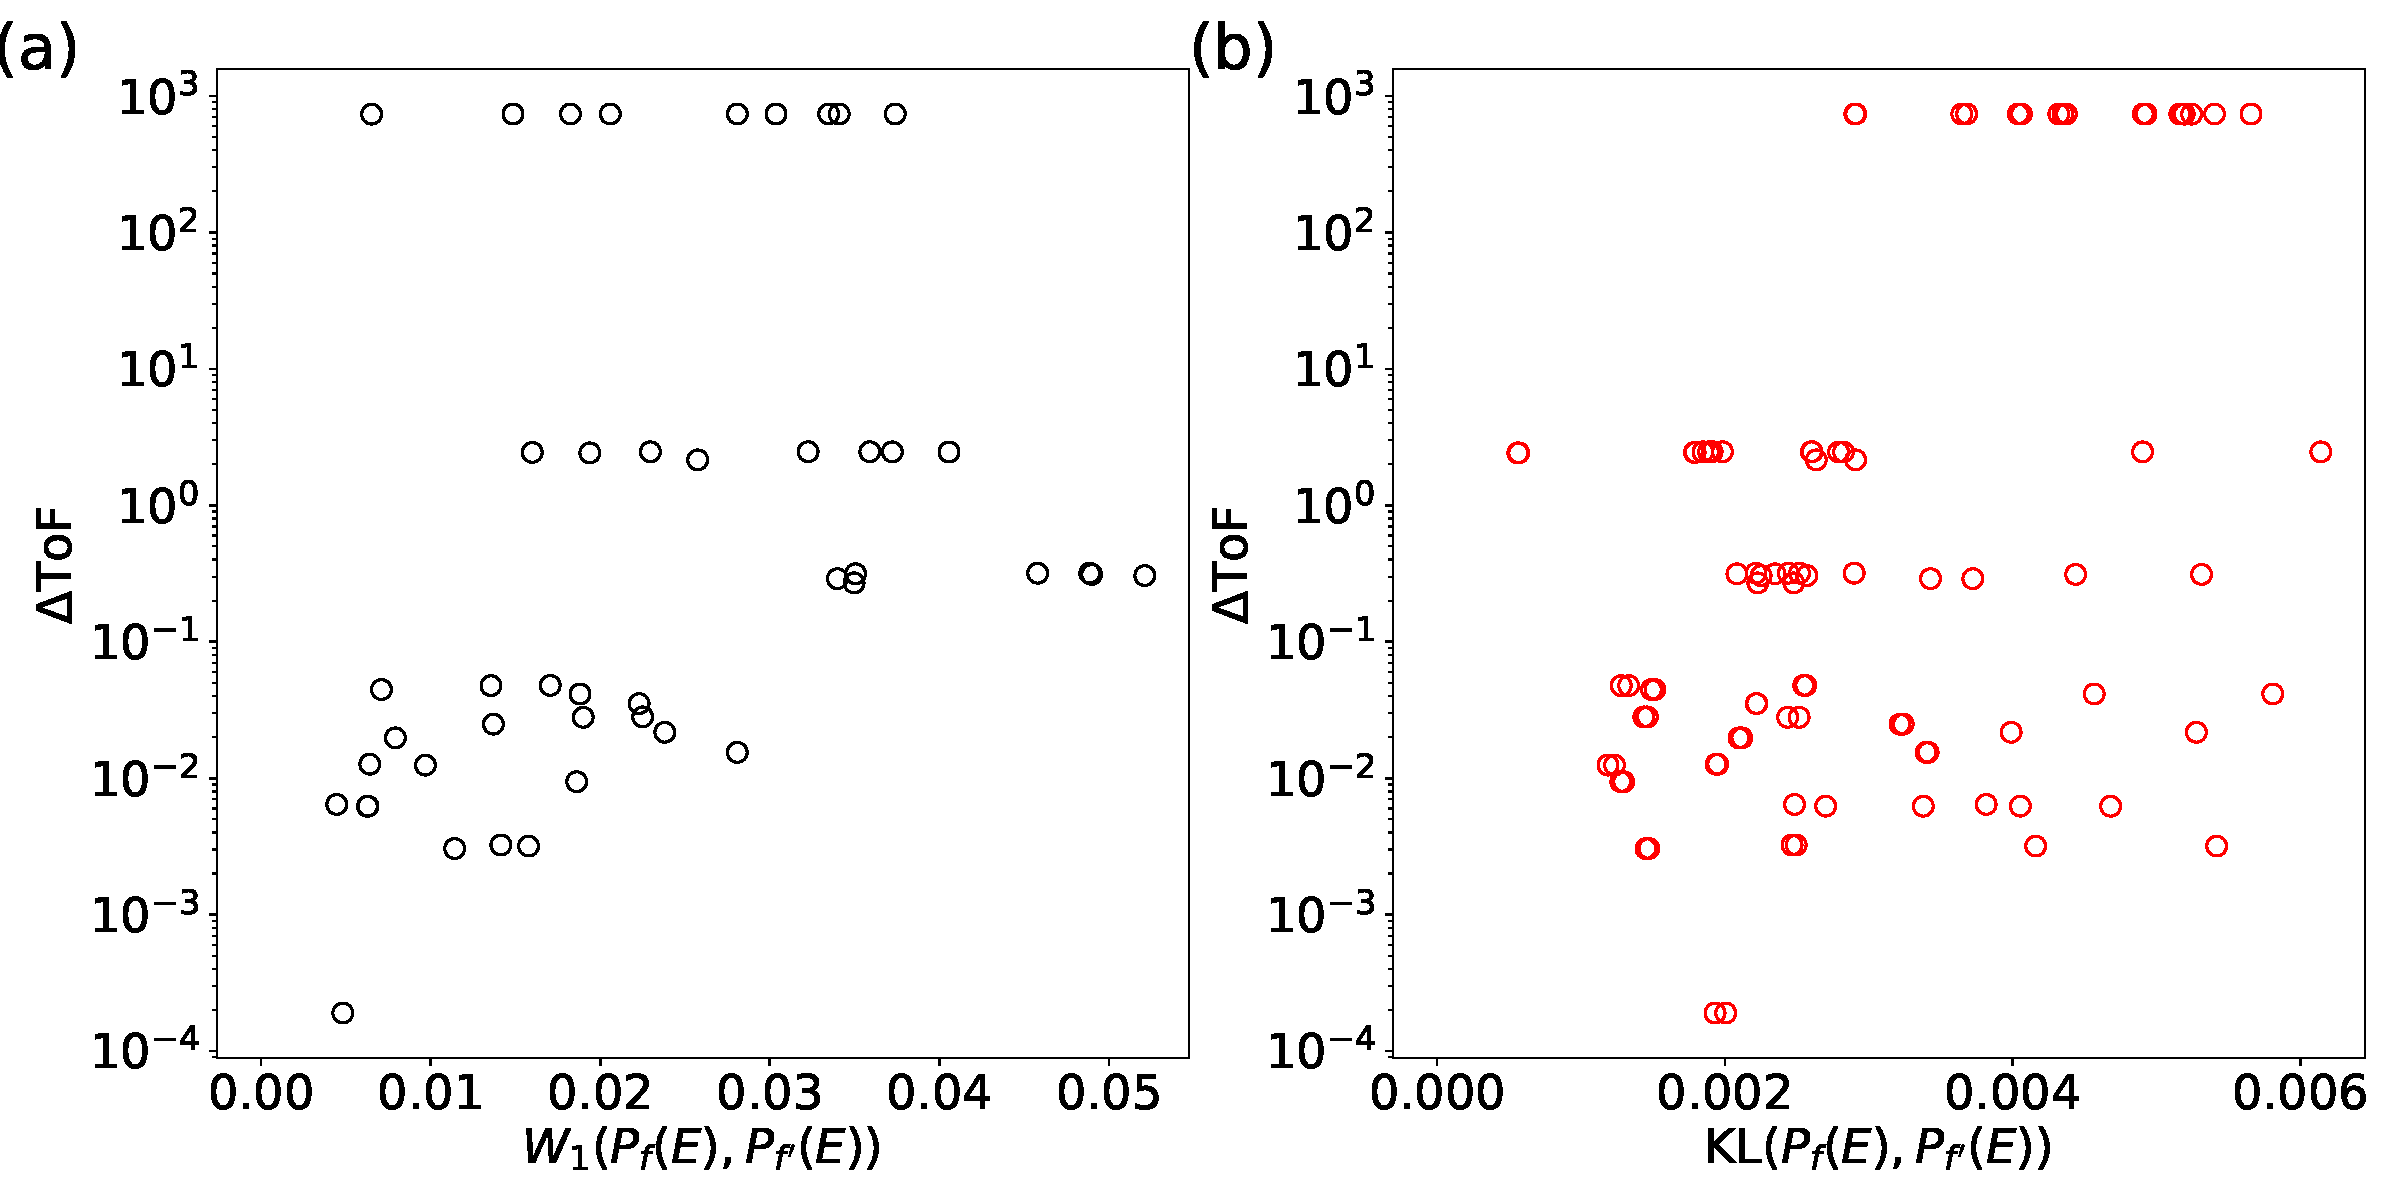
\includegraphics[width=0.9\textwidth]{figs/DeltaToF_W_KL_E.pdf}
    \caption{Left: scatter plot of $W_1(P_f,P_{f'})$ vs. $\Delta$ToF. Right: scatter plot of $KL(P_f(E),P_{f'}(E))$ vs. $\Delta$ToF.}
    \label{fig:distance_ToF}
\end{figure}

\textbf{Point 3:} We then examine other rate-related parameter distributions, calculating the Wasserstein distance and plotting against $\Delta$ToF. Figure \ref{fig:d_WD_tof} reveals that only the rate $P_f(\omega)$ has a large Wasserstein distance when varying $f^\text{DFT}$; other parameters show similar distributions.

\begin{figure}[h]
    \centering
    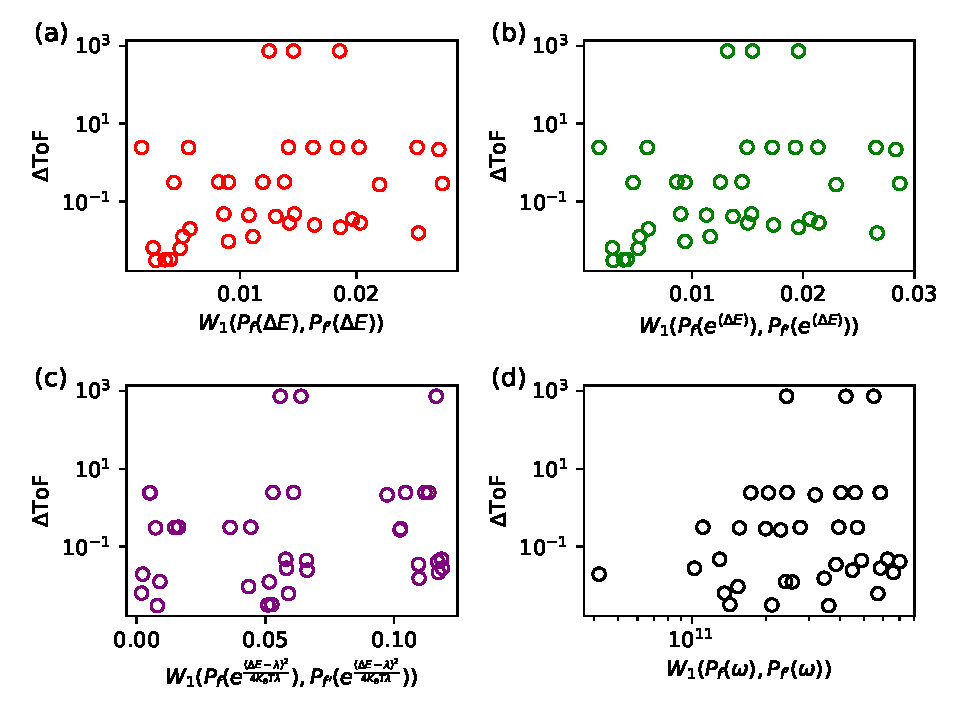
\includegraphics[width=0.7\textwidth]{figs/DeltaToF_W_all.pdf}
    \caption{Scatter plots of (a): $W_1(P_f(\Delta E),P_{f'}(\Delta E))$, (b): $W_1(P_f(\exp(\Delta E)),P_{f'}(\exp(\Delta E)))$, (c): $W_1(P_f(\exp \frac{-(\Delta E - \lambda)^2}{4 k_B T \lambda}),P_{f'}(\exp \frac{-(\Delta E - \lambda)^2}{4 k_B T \lambda}))$, and (d): $W_1 (P_f(\omega), P_{f'}(\omega) )$ vs. $\Delta$ToF.}
    \label{fig:d_WD_tof}
\end{figure}


\textbf{Point4:} Although $f^\text{DFT}$ affects $P_f(\omega)$, but we further notice that $\Delta$ToF is not correlated to its Wasserstein distance. 
So we hypothesize that the connectivity of the graph changed due to different $f^\text{DFT}$. The connectivity of the graph is quantified by the second eigenvector of the graph Laplacian, so we make the figure to investigate the correlation between the $\Delta$ToF and the graph connectivity. 
Figure .\ref{fig:d_eig_tof} shows the ratio of $f^\text{DFT}$ and the second eigenvalue ratio between the graph Laplacian. These two quantities look correlated, and we calculate the Spearman rank coefficient, which is shown in Table.\ref{tab:spearman}.

\begin{table}[h]
    \centering
    \begin{tabular}{c c c}
    \hline
        Data Set & Spearman Rank Coefficient & $p$-value \\ 
        \hline
        $\frac{\lambda_{2,L_W}(f)}{\lambda_{2,L_W}(f')}$ vs $\frac{\text{ToF}(f)}{\text{ToF}(f')}$ & -0.57 & 4.6e-5 \\
        $\frac{\lambda_{2,L_\text{rw}}(f)}{\lambda_{2,L_\text{rw}}(f')}$ vs $\frac{\text{ToF}(f)}{\text{ToF}(f')}$ & -0.38 & 9.4e-3 \\ 
    \hline
    \end{tabular}
    \caption{Spearman rank coefficients for the relationship between $\frac{\lambda_2(f)}{\lambda_2(f')}$ and $\frac{\text{ToF}(f)}{\text{ToF}(f')}$}
    \label{tab:spearman}
\end{table}

\begin{figure}[h]
    \centering
    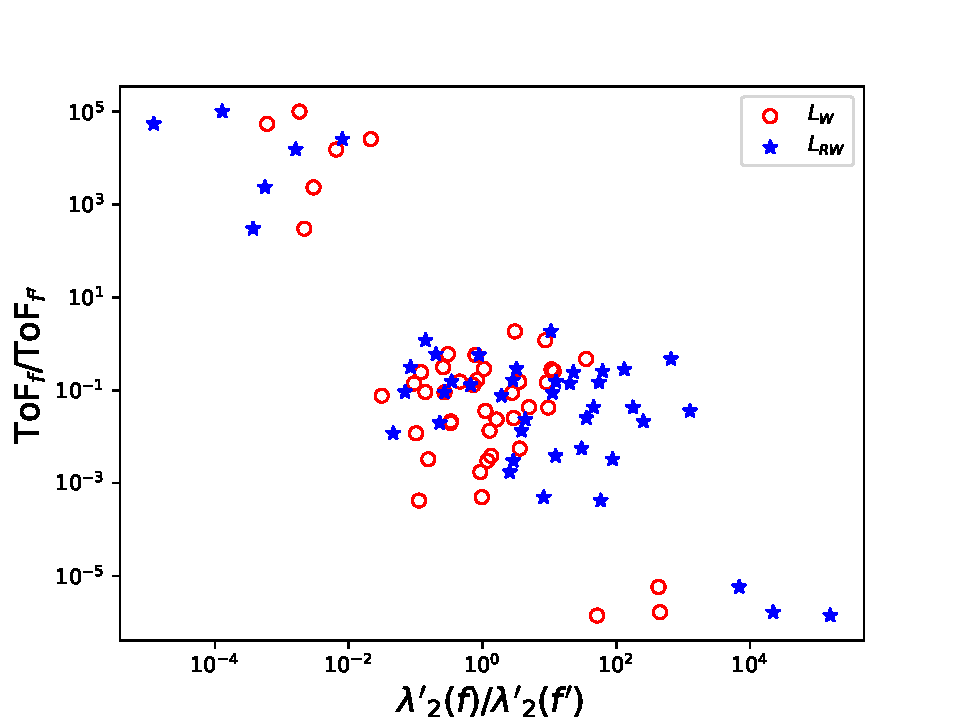
\includegraphics[width=0.6\textwidth]{figs/ratio_tof_2ndEigval.pdf}
    \caption{Scatter plot of $\frac{\lambda_{2}(f)}{\lambda_{2}(f')}$ vs. $\frac{\text{ToF}(f)}{\text{ToF}(f')}$}
    \label{fig:d_eig_tof}
\end{figure}


\textbf{Point5:} The eigenvalue comes in pair with the eigenvector, so we further investigated the corresponding second eigenvector element distributions, as shown in Fig.\ref{fig:2ndVecLW}. 
To our surprise, node 66 has very different second eigenvector entries, so we performed K-means partitioning on those second eigenvector elements.

\textbf{Point6:} After partitioning, we notice that the partition cost function is correlated to $\Delta$ToF.
This correlation shows that the $\Delta$ToF correlated to the connectivity of the graph, althouth the electronic structures and rate-related parameters are similar. 

\begin{figure}
    \centering
    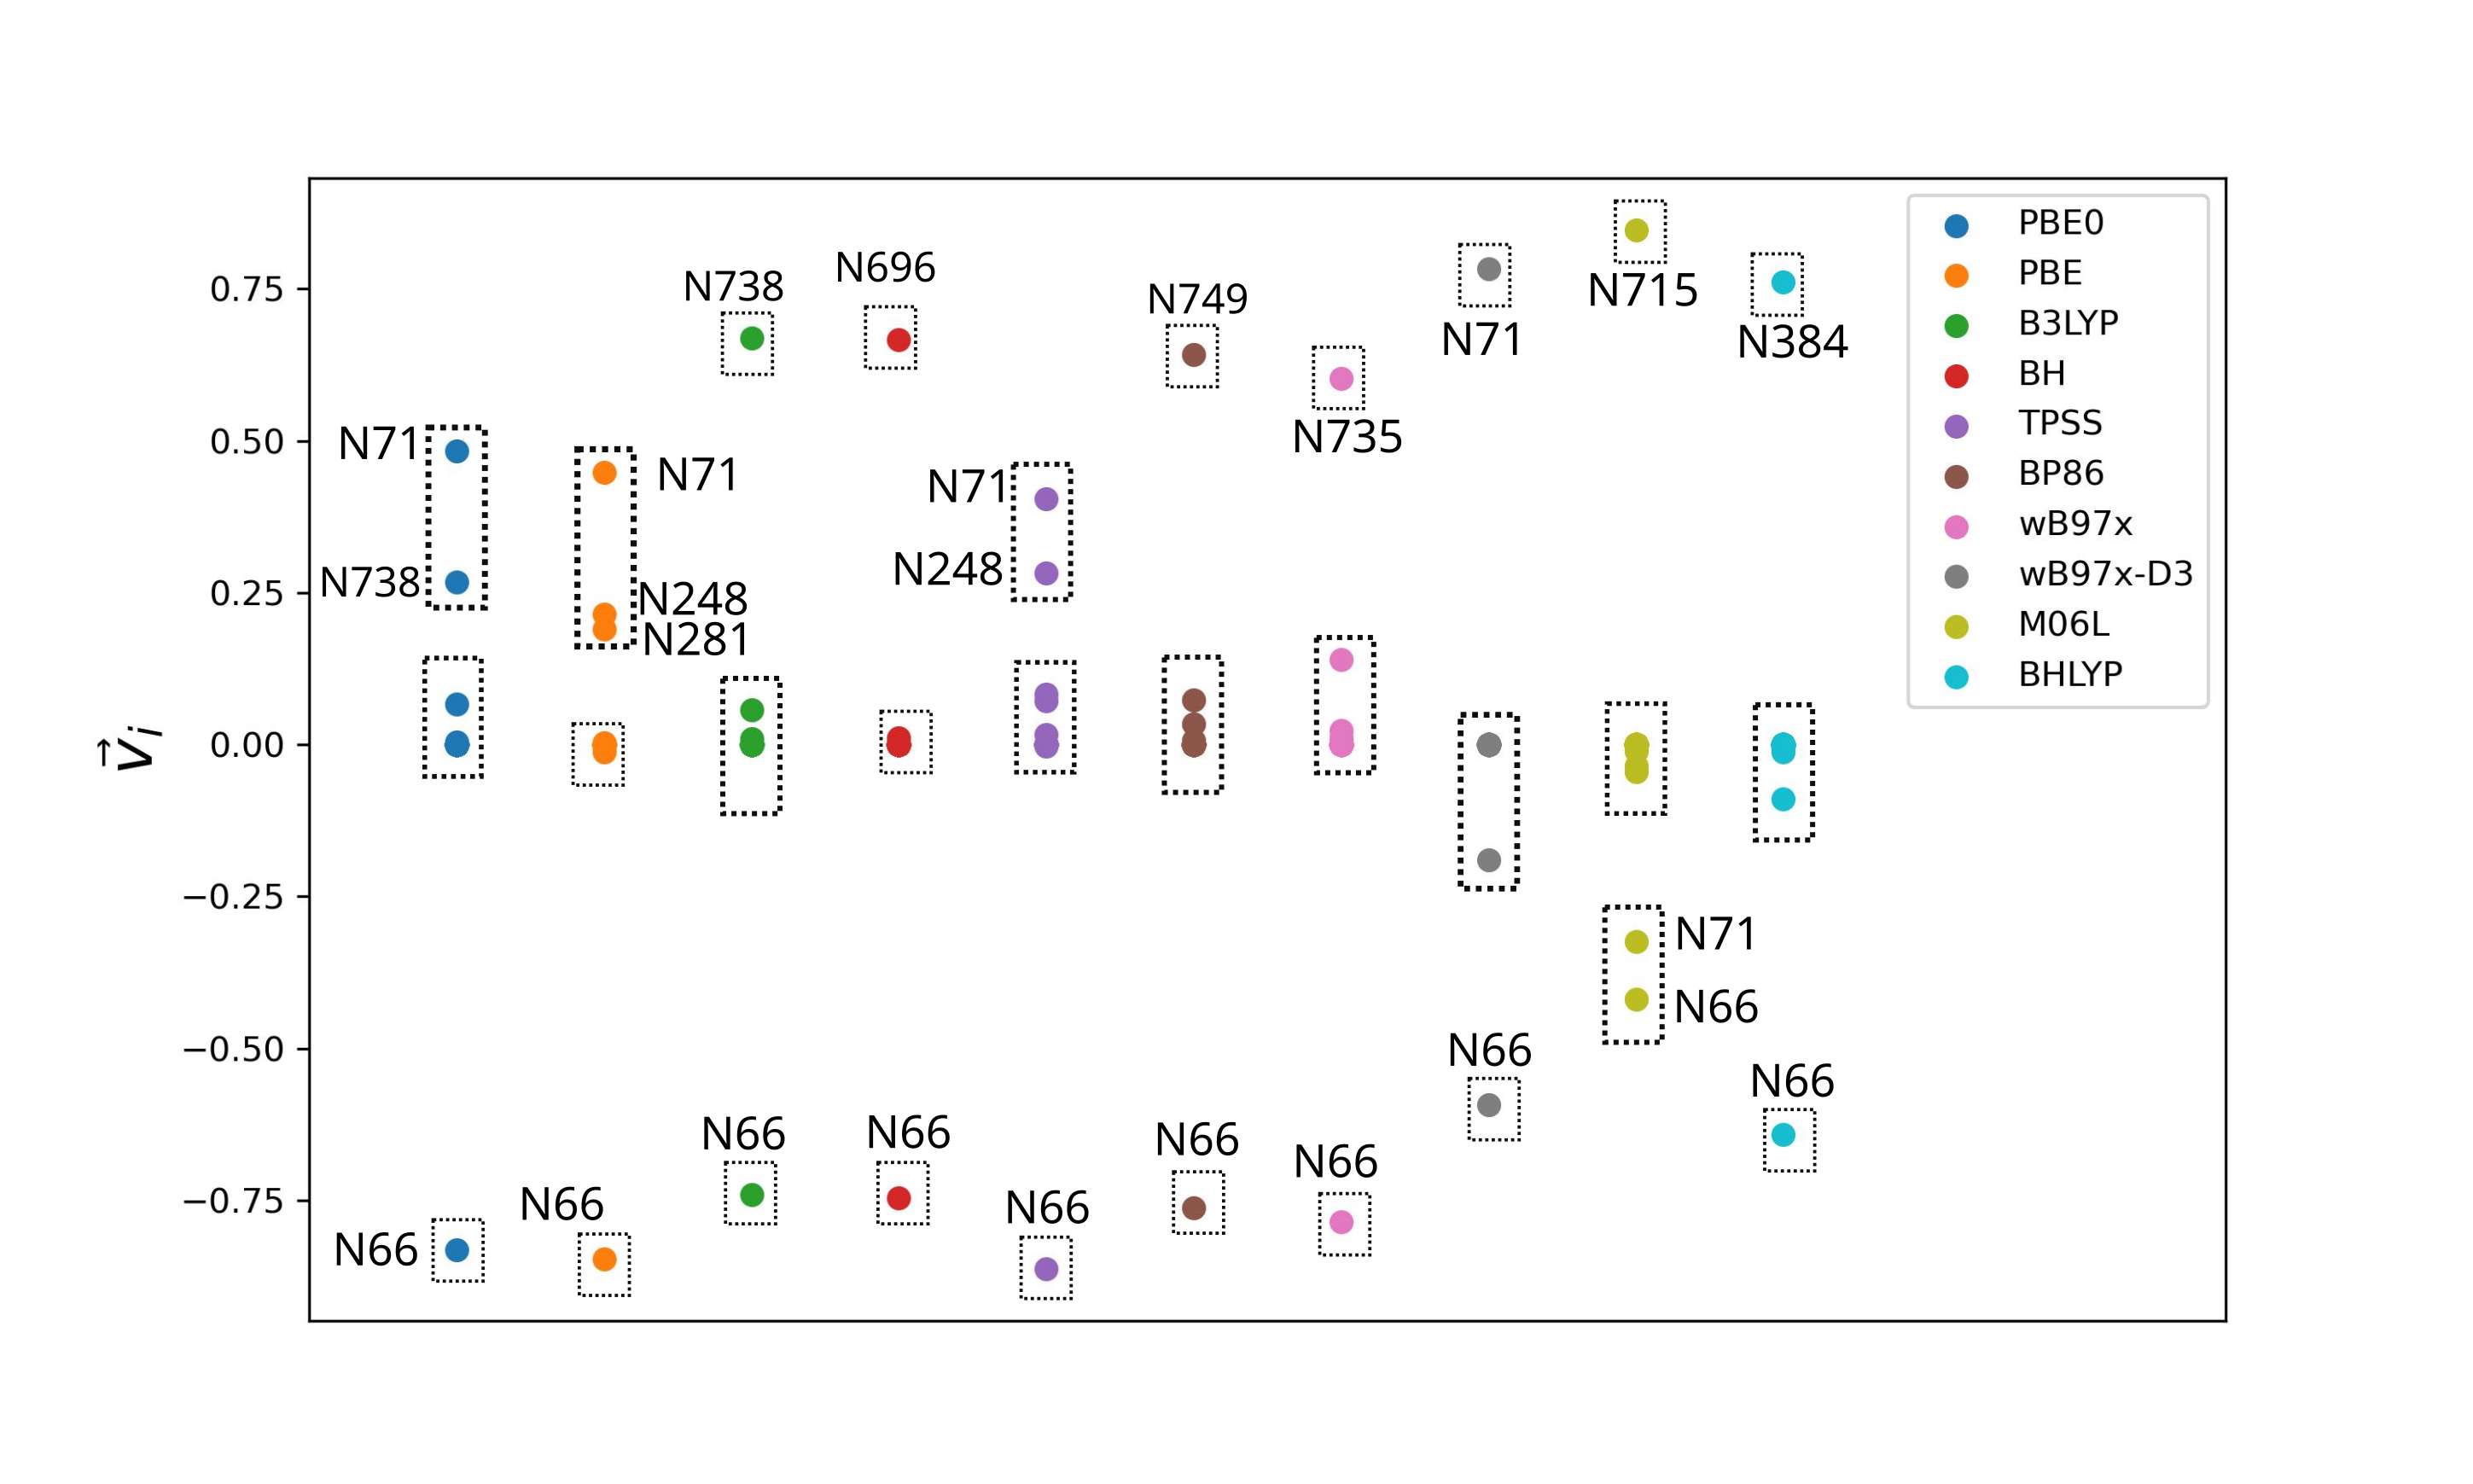
\includegraphics[width=0.8\textwidth]{figs/fig_2ndVecLw.png}
    \caption{Scatter plot of the eigen vector entries $\Vec{v}_i$ of $L_W$ for various $f$ indicated by the legend and point color. 
    The numbers are node index. The dash rectangular indicates the 3-means clusters that are detected as clusters by the Kmeans Lloyd's algorithm. }
    \label{fig:2ndVecLW}
\end{figure}

\begin{figure}
    \centering
    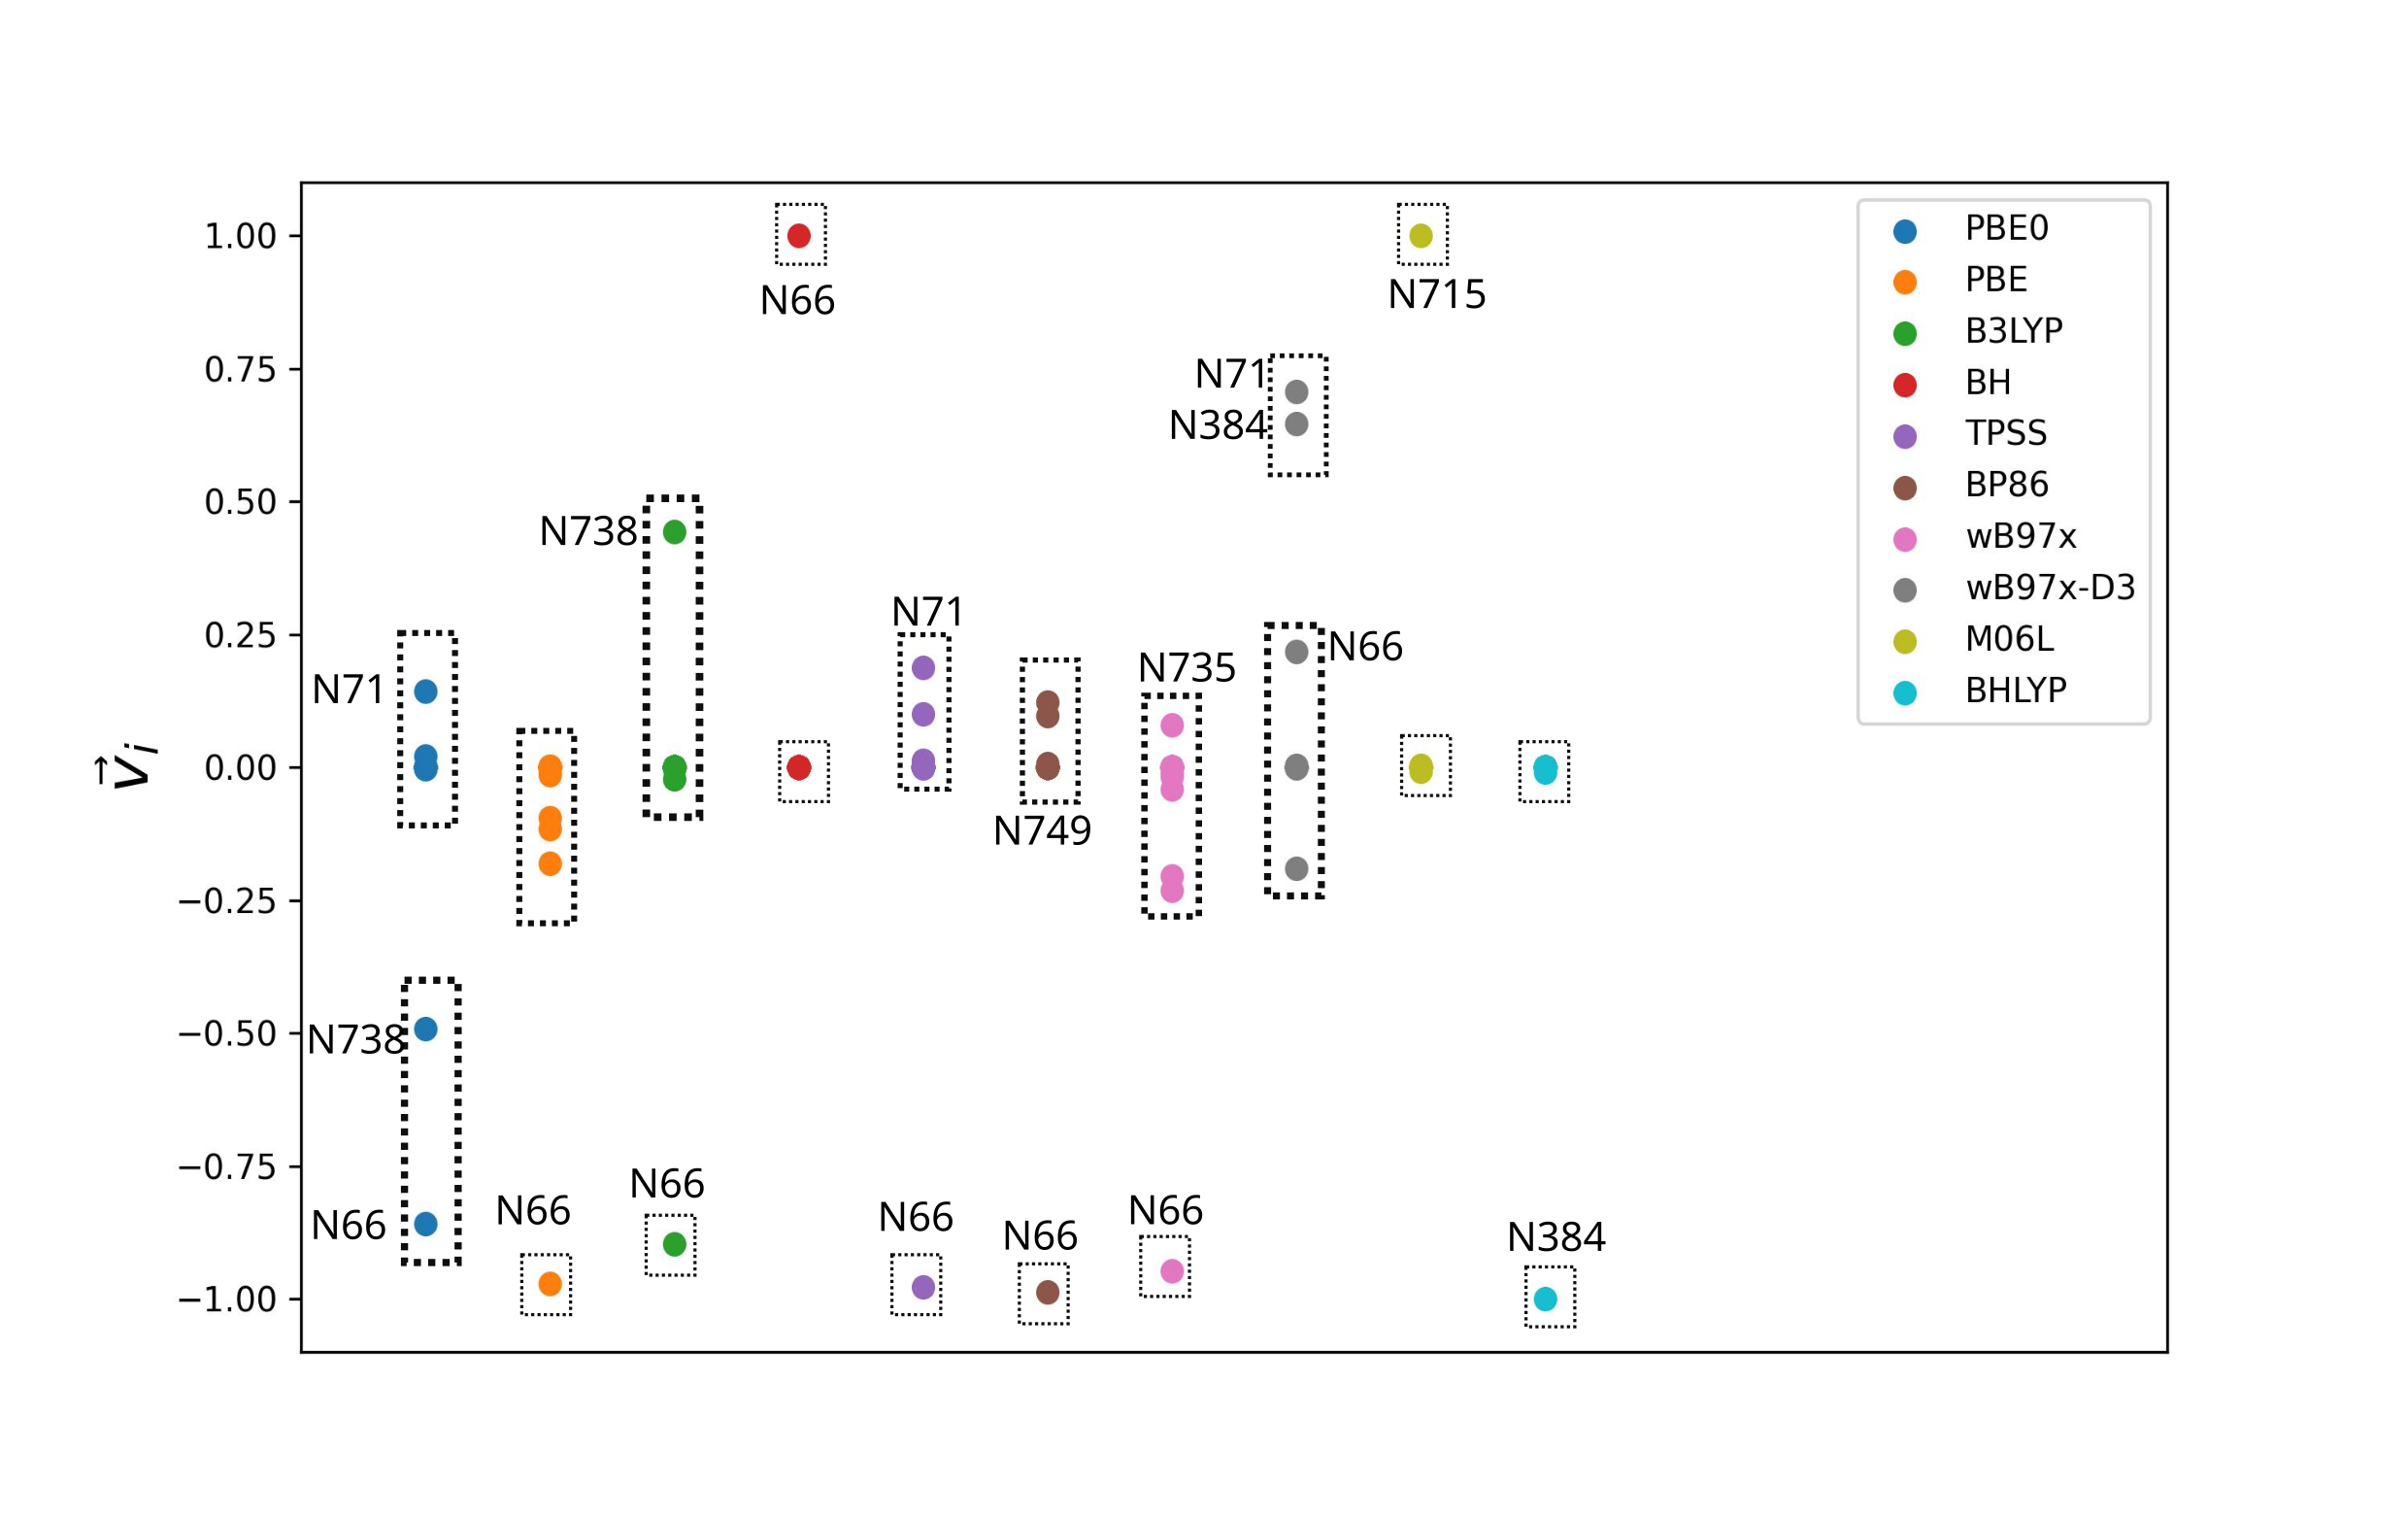
\includegraphics[width=0.8\textwidth]{figs/fig_2ndVecRW.png}
    \caption{Scatter plot of the eigen vector entries $\Vec{v}_i$ of $L_{rw}$ for various $f$ indicated by the legend and point color. 
    The numbers are node index. The dash rectangular indicates the 3-means clusters that are detected as clusters by the Kmeans Lloyd's algorithm.  }
    \label{fig:2ndVecRW}
\end{figure}


Figure \ref{fig:fig_Z_ToF} shows scatter plots of K-means clustering partition cost $Z_{2c}, Z_{3c}$ versus ToF. For the normal Laplacian $L_w$, $Z_{2c}$ is not correlated with the ToF, but $Z_{3c}$ is. For the Random-walk Laplacian, both $Z_{2c}$ and $Z_{3c}$ show a strong correlation with ToF. Thus, the clustering cost function indicates the speed of charge dynamics as measured by ToF.

\begin{figure}
    \centering
    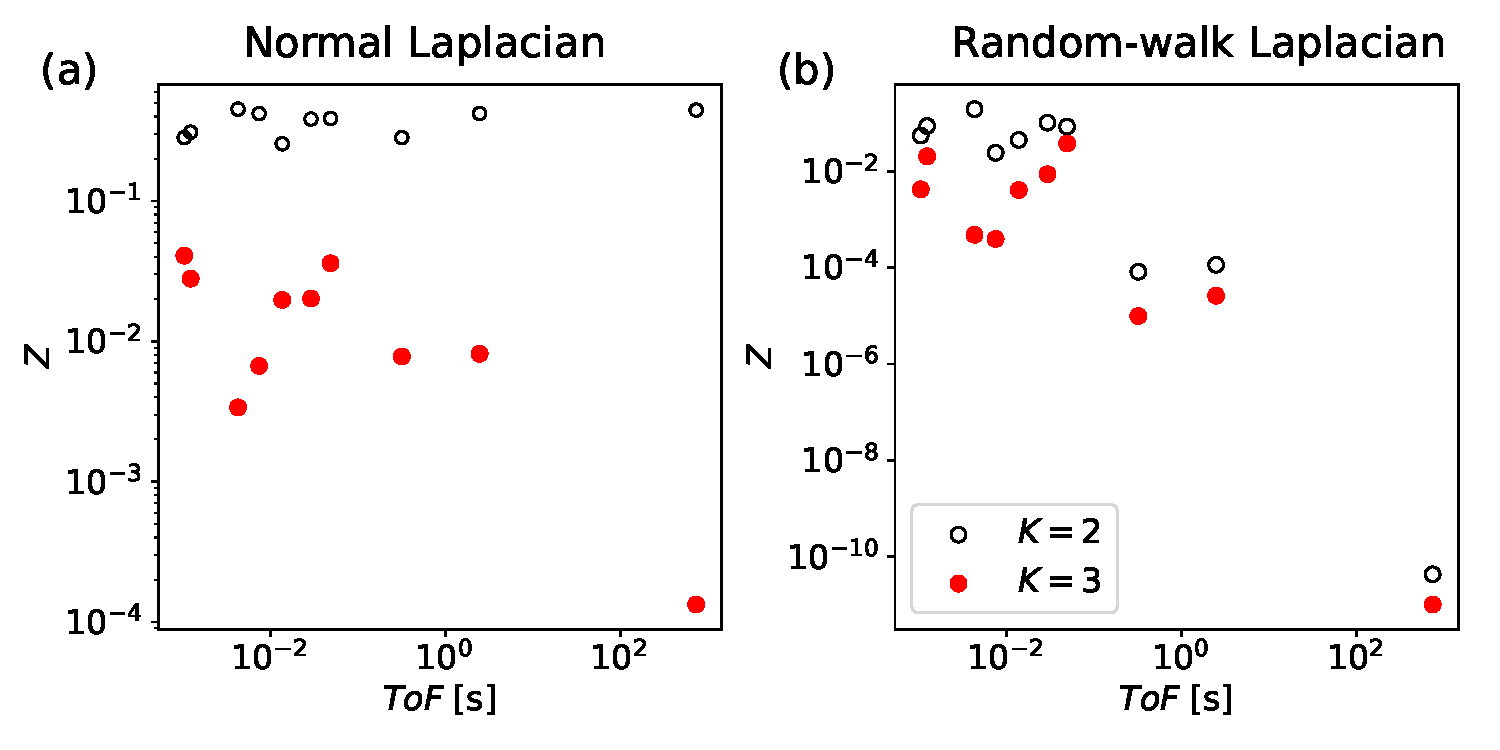
\includegraphics[width=0.9\textwidth]{figs/fig_Z_ToF.pdf}
    \caption{Scatter plot of $Z$ vs $\text{ToF}$. (a): K-means partition of the second eigenvector of $L_W$ for $K=2$ and $K=3$ (b) K-means partition of the second eigenvector of $L_{RW}$ for $K=2$ and $K=3$}
    \label{fig:fig_Z_ToF}
\end{figure} 


\textbf{Point7:} Now that the ToF has a large range, we want to know which ToF to trust.  And for application purposes, a very important message is to know what the range of ToF will give a 90\% confidence level. 

Since we do not really know the exchange-correlation potential, we assume that for each molecule, the uncertainty in its energy $E_i$ is represented by a normal distribution $E_i \in N(\bar{E_i},\sigma(E_i))$. Normal distribution is used because the normal distribution encodes the maximum amount of uncertainty over the real numbers out of all possible probability distributions with the same variance. 
So the normal distribution inserts the least amount of prior knowledge into our model. 
So we experiment: 

\textbf{Point8:} For each molecule energy $E_i$, we use maximum likelihood estimation to obtain the $N(\bar{E_i},\sigma(E_i))$. Then use sample a set of $E_i$ and calculate the ToF, with $\lambda,J_{i,j}$ fixed at the average values. 
Repeat the $E_i$ sampling and ToF calculation for 100000 times, and plot ToF distribution. This process is called the Monte Carlo sampling. 

Similarly, for $\lambda,J_{i,j}$, we perform the Monte Carlo sampling as been done for $E_i$. The resulting ToF is shown in Fig.\ref{fig:ToFs}.

\begin{figure}
    \centering
    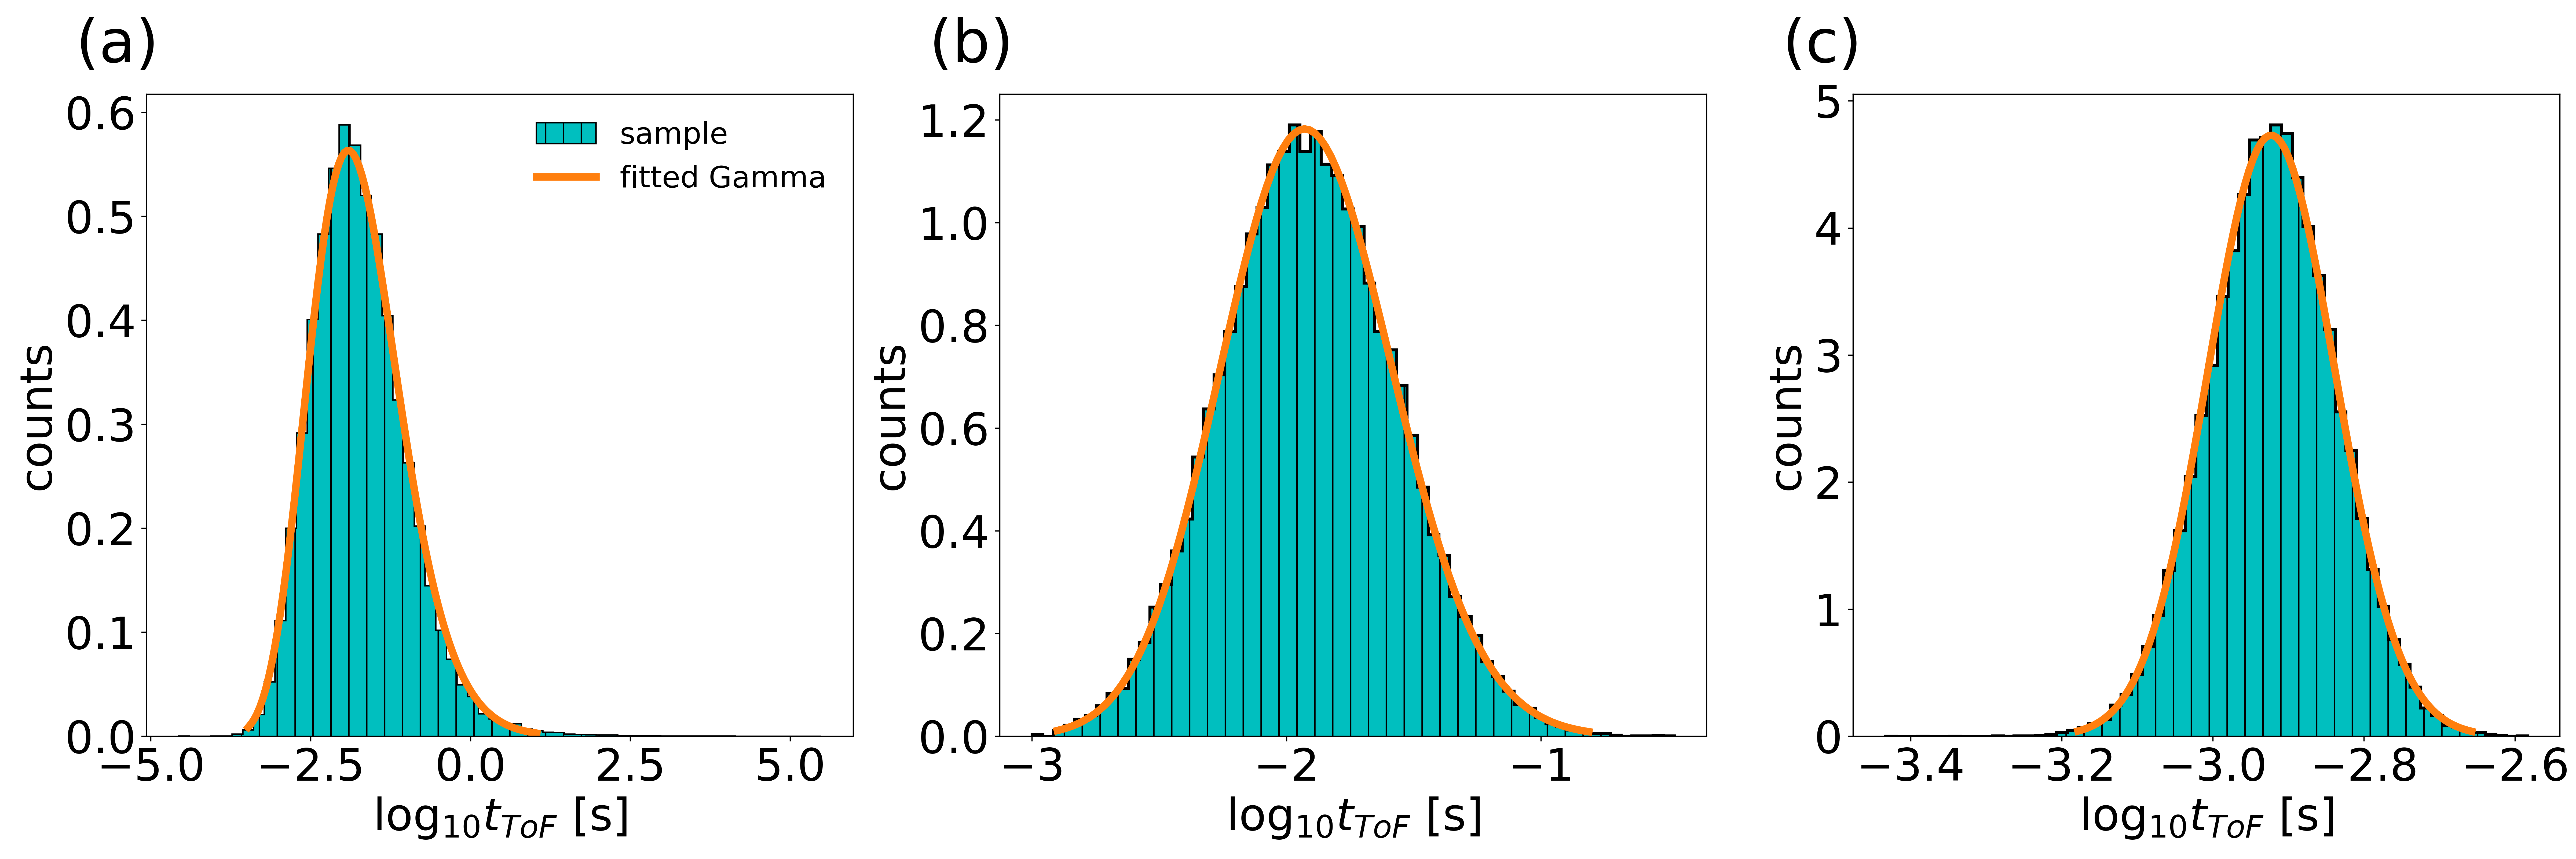
\includegraphics[width=0.9\textwidth]{figs/fig_mle.png}
    \caption{(a)The ToF distribution for 100000 samples where each $E_i$ is drawn from $N(\bar{E}_i,\sigma(E_i))$. The red curve is fitted to a gamma distribution. (b)The ToF distribution for 100000 samples where each $\lambda$ is drawn from $N(\bar{\lambda},\sigma(\lambda))$.(c)The ToF distribution for 100000 samples when each $J_{i,j}$ is drawn from $N(\bar{J_{i,j}},\sigma(J_{i,j}))$.}
    \label{fig:ToFs}
\end{figure} 

This figure shows that ToF is more sensitive to change in $E_i$ and least sensitive to $J_{i,j}$, even though from the scatter plots Fig.\ref{fig:scatterJ} the $J_{i,j}$ has a very large magnitude deviation. 

The dataset of $\log_{10}(\text{ToF})$ can be well-fitted to a Gamma distribution. 
The statistical calculation has results:
\begin{itemize}
    \item When $E_i \in N(\bar{E_i},\sigma(E_i))$, the $\log_{10}(\text{ToF})$ has mean -1.73 and a standard deviation of 0.73.
    \item When $\lambda \in N(\bar{\lambda},\sigma(\lambda))$, the $\log_{10}(\text{ToF})$ has mean -1.91 and a standard deviation of 0.34.
    \item When $J_{i,j} \in N(\bar{J_{i,j}},\sigma(J_{i,j}))$, the $\log_{10}(\text{ToF})$ has mean -2.92 and a standard deviation of 0.08.
\end{itemize}

When we use $E_i \in N(\bar{E_i},\sigma(E_i))$, $\lambda \in N(\bar{\lambda},\sigma(\lambda))$, $J_{i,j} \in N(\bar{J_{i,j}},\sigma(J_{i,j}))$ at the same to perform the Monte Carlo sampling of ToF calculation, the ToF is shown in Fig.\ref{fig:ToFs2}. the $\log_{10}(\text{ToF})$ has mean -2.72 and a standard deviation of 0.80. To obtain a 90\% confidence level, then $-3.93 < \log_{10}(\text{ToF}) < -1.30$.
\begin{figure}
    \centering
    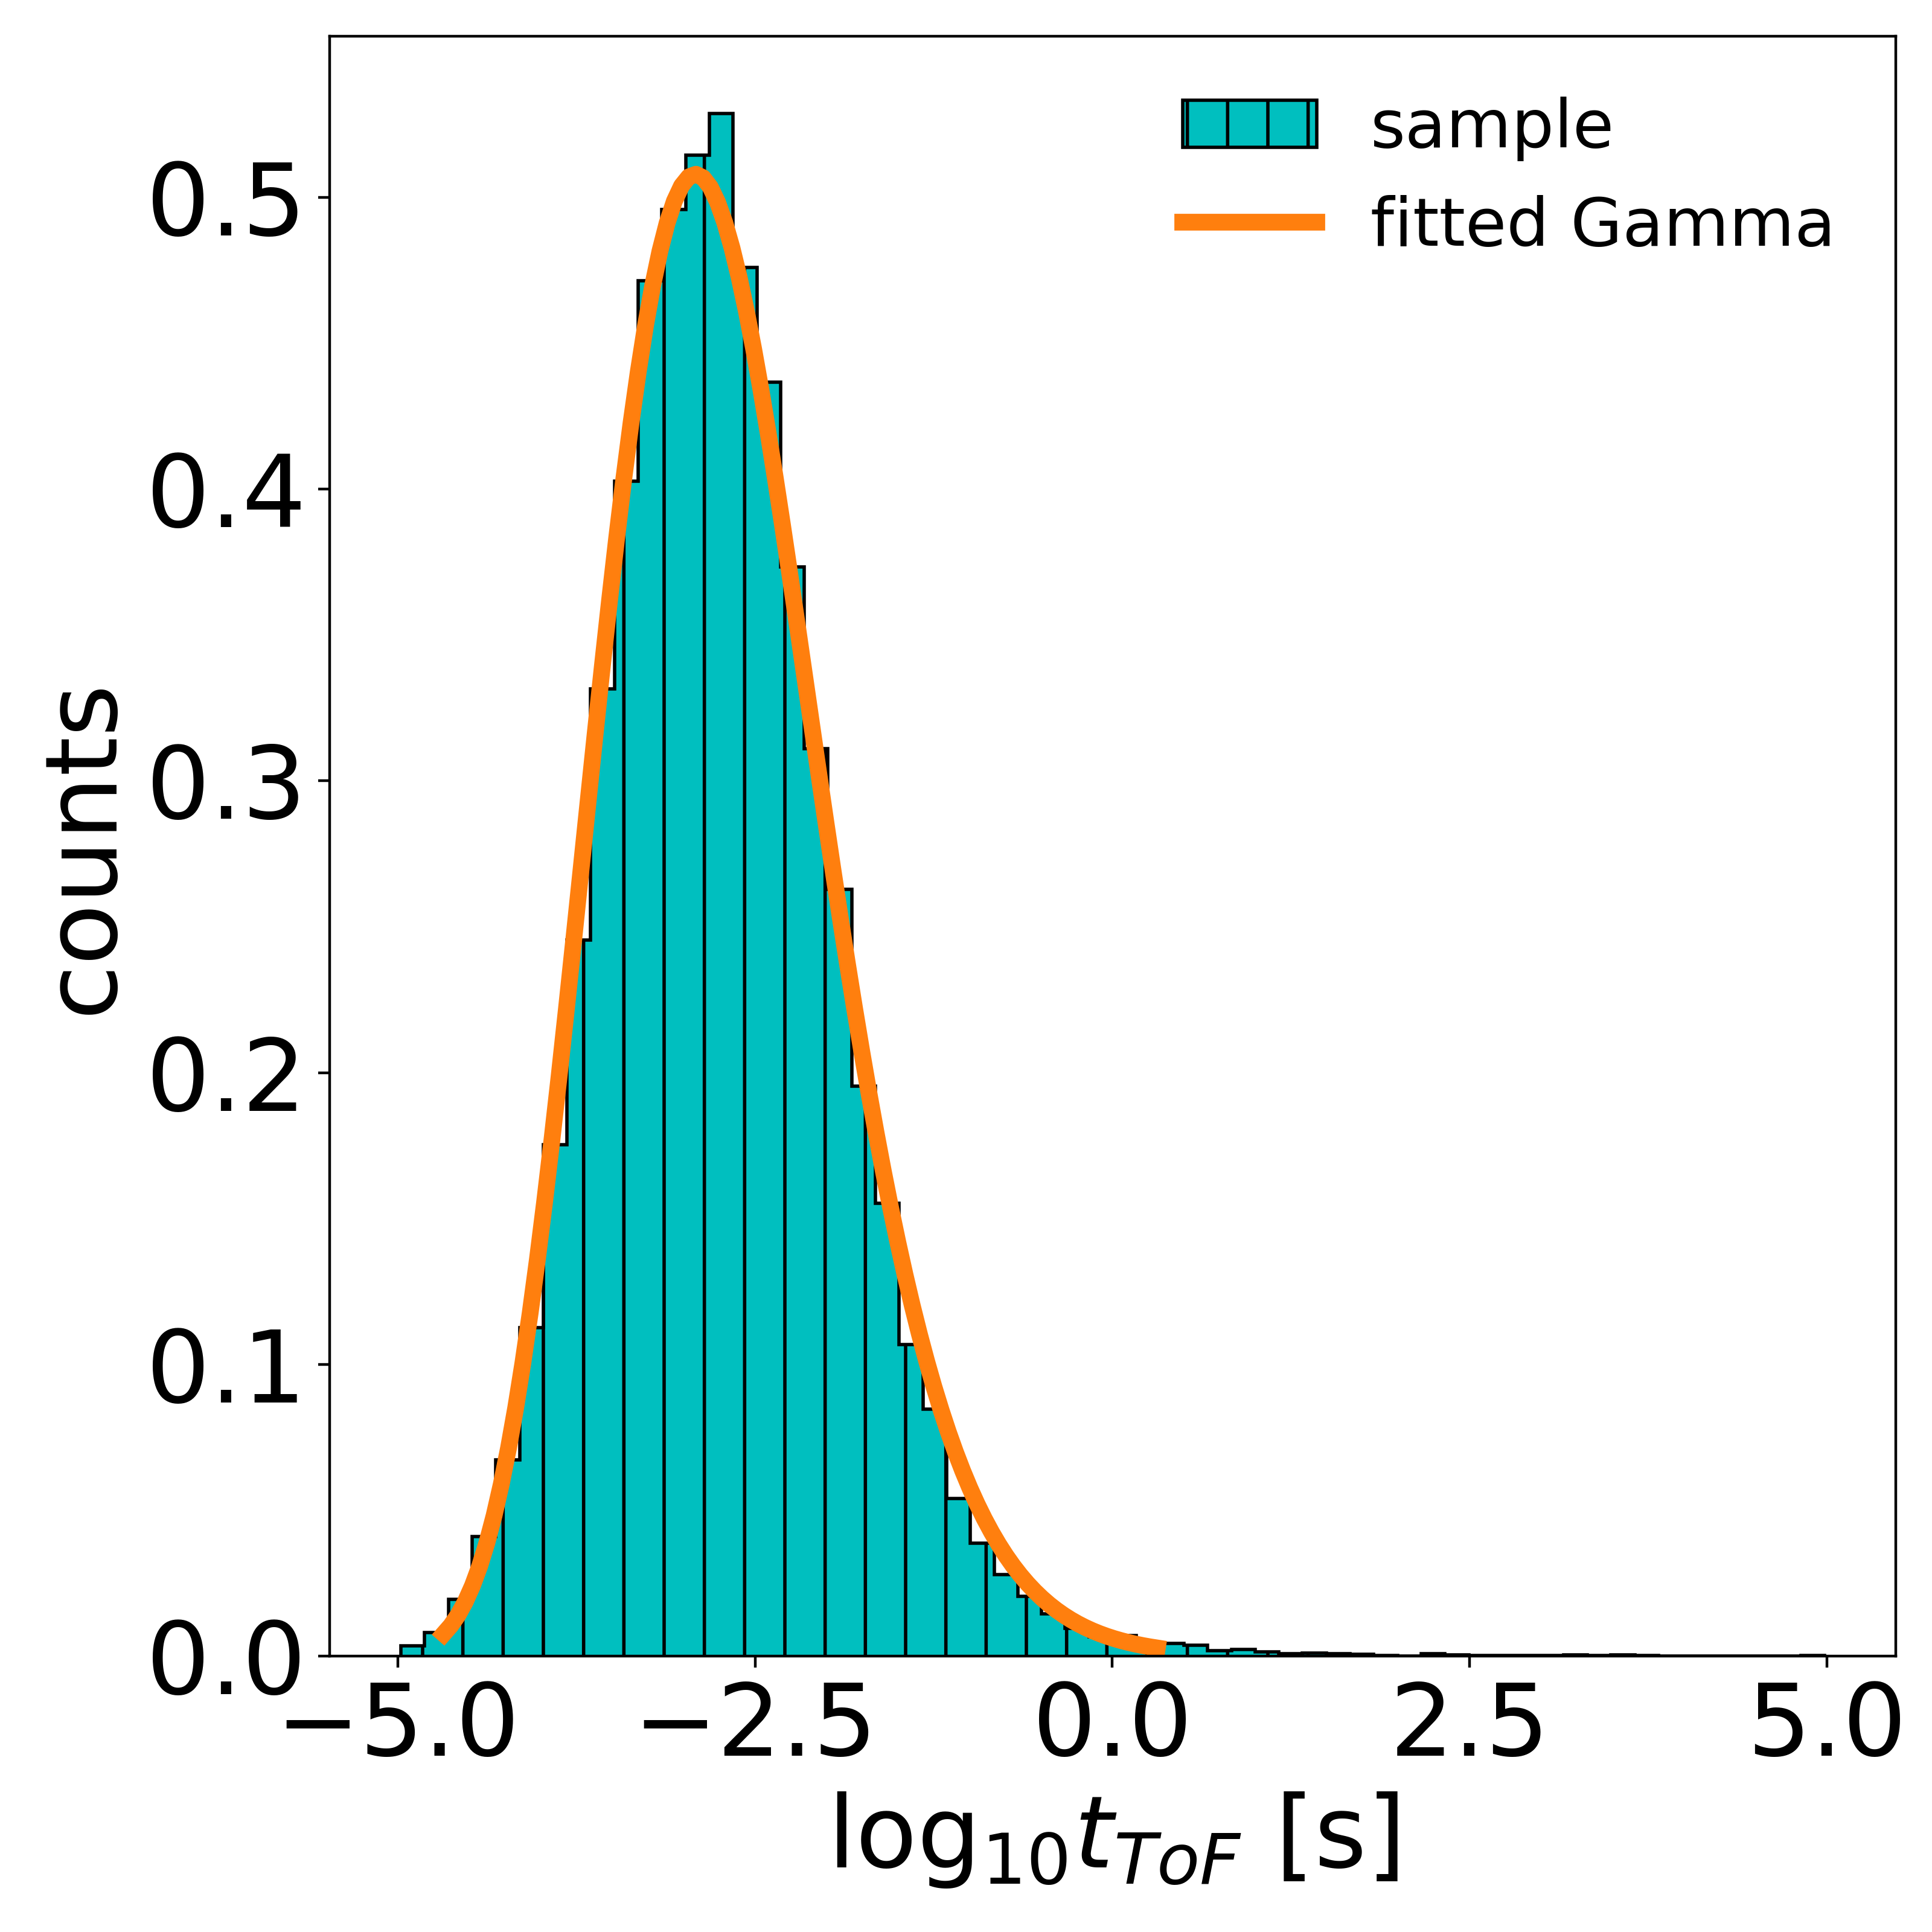
\includegraphics[width=0.6\textwidth]{figs/fig_mle2.png}
    \caption{The ToF distribution for 100000 samples where each $E_i$ is drawn from $N(\bar{E}_i,\sigma(E_i))$, $\lambda$ is drawn from $N(\bar{\lambda},\sigma(\lambda))$, and each $J_{i,j}$ is drawn from $N(\bar{J_{i,j}},\sigma(J_{i,j}))$. The red curve is fitted to a gamma distribution.}
    \label{fig:ToFs2}
\end{figure} 

\section{Uncertainty in ToF}
Now we need to answer which ToF is accurate. 
Using the multiscale model to determine the ToF is a function $f: \mathbb{R}^d \rightarrow \mathbb{R}^+$, which maps the parameter vector $$\vec{x} = [ E_1,E_2,\cdots,E_N, R_1,R_2,\cdots,R_N,J_1,J_2,\cdots,J_{N_\text{pair}} ]$$ to a real value $\tau \in \mathbb{R}^+$.

Due to noise and approximation in the multiscale model, each element in $\vec{x}$ can be considered as an exact value plus an error term, for example $$E_1 = \hat{E}_1 + \epsilon_{E_1} $$
There is no prior knowledge about this error terms. 
Since the normal distribution inserts the least amount of prior knowledge into a model and encodes the maximum amount of uncertainty, we want to quantify the uncertainty when those error terms are normally distributed. 
\end{comment}


\end{document}
